\documentclass[preprintnumbers,amsmath,amssymb,superscriptaddress,twocolumn,showpacs]{revtex4-2}
\usepackage{graphicx}% Include figure files
\usepackage{dcolumn}% Align table columns on decimal point
\usepackage{bm}% bold math
\usepackage{physics}
\usepackage[caption=false]{subfig}



\def\sgn{\mathop{\rm sgn}}
\newcommand{\be}{\begin{equation}}
\newcommand{\ee}{\end{equation}}
\newcommand{\bea}{\begin{eqnarray}}
\newcommand{\eea}{\end{eqnarray}}

\begin{document}

\title{Depolarization of interacting NV$^-$ centers at low magnetic fields}

\author{C. Pellet-Mary$^1$, M. Perdriat$^1$, P. Huillery$^2$,  G. H\'etet} 

\affiliation{Laboratoire De Physique de l'\'Ecole Normale Sup\'erieure, \'Ecole Normale Sup\'erieure, PSL Research University, CNRS, Sorbonne Universit\'e, Universit\'e Paris Cit\'e , 24 rue Lhomond, 75231 Paris Cedex 05, France \\ $^2$ Univ Rennes, INSA Rennes, CNRS, Institut FOTON - UMR 6082, F-35000 Rennes, France}

\begin{abstract}
We study dipolar interaction processes in dense ensembles of negatively charged nitrogen vacancy (NV$^-$) centers under small magnetic fields. Employing magnetic field scans close to zero-field along specific crystalline direction while recording the NV$^-$ spin relaxation rate, we could identify regimes where flip-flop, double-flip processes as well as mixing induced by local electric field play a role in the NV-NV cross-relaxation .
Our results are relevant for understanding decoherence in many-body spin systems as well as for high sensitivity magneto- and electro-metry with long-lived interacting solid-state spins. As a proof of principle, we present an orientation and microwave-free magnetometer based on cross-relaxation, and operating with a sensitivity below $100$ nT/$\sqrt{\rm Hz}$.
\end{abstract}

\maketitle

The electronic spin properties of the negatively charged nitrogen-vacancy (NV$^-$) center in diamond has given rise to a wealth of applications in nanoscale sensing and quantum information science thanks in part to the possibility to optically polarize and read-out its spin state at ambient conditions \cite{DOHERTY20131}. In particular, ensembles of NV centers are widely studied for their enhanced magnetic field sensing capabilities \cite{Acosta, TALLAIRE2020421,edmonds2021characterisation, chatzidrosos2021fiberized} and as pristine platforms for studying many body effects \citep{kucsko2018critical, ChoiNat, ZuYao}. When the NV spin concentration reaches ppm values, spin depolarisation, or cross-relaxation (CR) takes place through a very rich many body dynamics associated with disorder \citep{choi_observation_2017}. These mechanisms however limit the efficiency of typical microwave based NV magnetometers, but can be harnessed to attain sub-heisenberg limited magnetometers \citep{zhou2020quantum}. Further, CR mechanisms can be turned as a tool for magnetic field sensing \cite{akhmedzhanov_microwave-free_2017, akhmedzhanov_magnetometry_2019}. 
Spectral features in the photoluminescence (PL) indeed appear when the magnetic field crosses specific crystal planes where dipolar interactions are enhanced, leading to CR. The projected sensitivity of such magnetometers lie in the tens of pT$/\sqrt{\rm Hz}$  \cite{akhmedzhanov_microwave-free_2017}, on a par with the most sensitive microwave based NV magnetometers \cite{Wolf, Sturner}. 

CR features at zero-field have also been observed and could also be deployed for high sensitivity microwave free magnetometry.
The CR contrast was indeed shown to be much stronger \citep{jarmola_longitudinal_2015,  mrozek_longitudinal_2015}. However all the relaxation mechanisms at these low field levels have not been identified. 
Here, we study dipolar interaction processes in ensembles of NV centers under small magnetic fields. Specifically, by employing magnetic field scans along specific crystalline directions, we identify regimes where flip-flop, double-flip processes as well as mixing induced by local electric field play a role in the CR. We also present an orientation and microwave-free magnetometer operating with a sensitivity below $100$ nT/$\sqrt{\rm Hz}$ at zero-field, where double-flip processes amongst NV centers dominate.

\begin{figure}
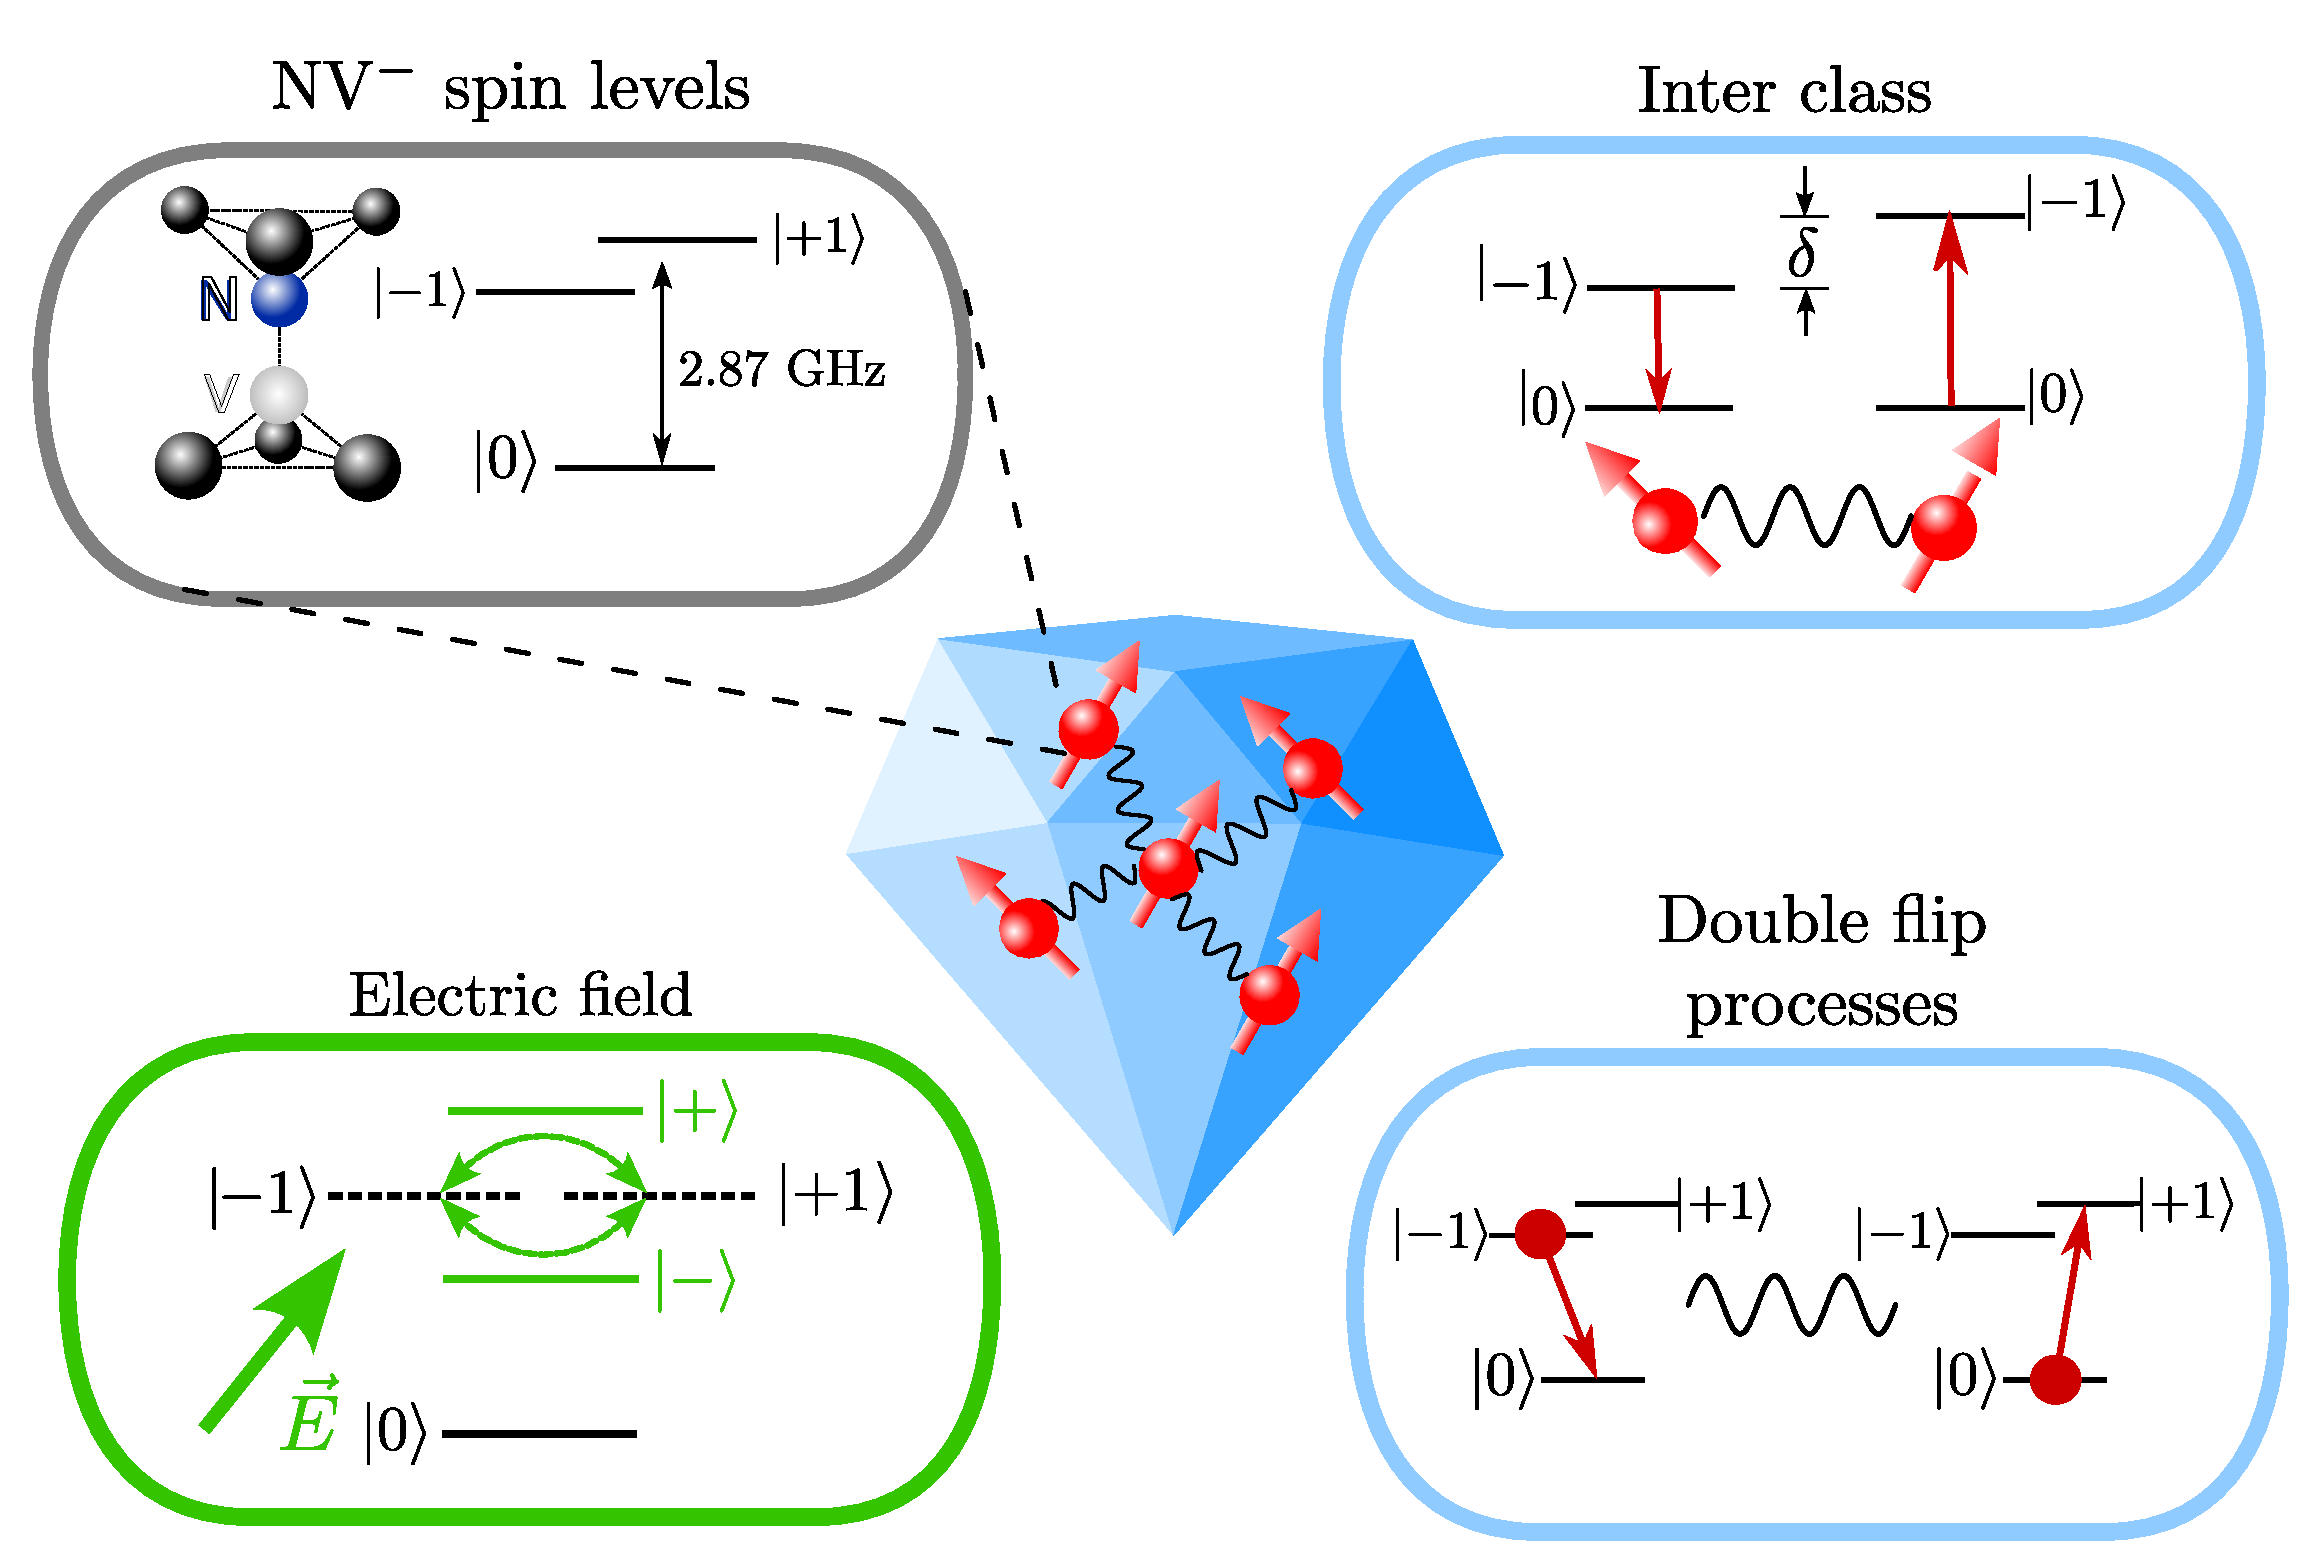
\includegraphics[width=0.45\textwidth]{Figures/shema_summary.pdf}
\caption{Schematics showing a diamond with interacting spins as well as the three processes that can account for dipolar relaxation :flip-flop processes involving two different classes of NV centers, local electric field mixing and double-flip processes where two units of spin angular momentum are exchanged. }
\label{schema_intro}
\end{figure}

The electronic spin of NV center is a spin-1 system in the electronic ground state (see Fig. 1, top left panel), which can be optically polarized in the $\ket{m_s=0}$ state. The PL of this state is also larger than in the $\ket{m_s=\pm 1}$ states enabling spin-read out at ambient temperature \cite{DOHERTY20131}. The $\ket{m_s=\pm 1}$ spin states are separated from the $\ket{m_s=0}$ state by  $D = (2\pi) 2.87$ GHz so that when a resonant microwave or static transverse magnetic field is applied, the PL is reduced \citep{epstein2005anisotropic,lai2009influence}.  The processes that lead to CR in such a spin-1 system are depicted in Fig.~1. Flip-flop processes involving coupling between NV centers from identical or from different orientations are depicted in the top-right panel. They have already been shown to play a dominant role when tuning $\delta$ {\it via} longitudinal B fields scans, when $B \gtrsim 30$G \cite{choi_observation_2017}. We will show here that under smaller magnetic fields or using purely transverse fields, double-flip up and down as well as the mixing induced by local electric field give a significant contribution to the CR (two bottom panels). 

Fig.  \ref{T1}-a) and b) show the change in PL as a function of an external magnetic field for two samples with a low and high concentration of NV$^-$ centers respectively, detailed in the supplementary material (SM sec. II) of this article \citep{SI_low_filed_CR} \nocite{anishchik2015low, filimonenko2020weak, van1990electric}. Both samples show a decrease in PL as the magnetic field amplitude increases.  There is however a stark difference in the low magnetic field region where only high-density samples shows a drop in PL \citep{jarmola_longitudinal_2015,  mrozek_longitudinal_2015}. This effect can be observed on all our samples whenever the NV concentration lies in the ppm range. The drop of the PL at low magnetic field was shown to be associated with a decrease of the NV's spin lifetime $T_1$ \citep{jarmola_temperature-_2012}, which results in a decrease of the population in the bright state $\ket{0}$.

The depolarization dynamics of the NV spins for single or dilute ensembles of NV centers at room temperature is dominated by two-phonon Raman processes \citep{redman1991spin,jarmola_temperature-_2012,norambuena2018spin}, which depend on the crystal lattice temperature. It has been observed that dense NV centers ensembles in fact  have an additional spin decay channel \citep{jarmola_temperature-_2012,jarmola_longitudinal_2015,mrozek_longitudinal_2015, choi2017depolarization, akhmedzhanov_microwave-free_2017, akhmedzhanov_magnetometry_2019, pellet2021magnetic, mrozek2021characterization}, which depends greatly on the magnetic field amplitude. This effect has been attributed to CR between the NV centers through dipole-dipole coupling \citep{mrozek_longitudinal_2015, choi2017depolarization}. 
The reason is that at zero-field many NV ``classes" - that is physical orientation of the NV axis is the diamond crystal cell - becomes resonant, which increases the dipolar relaxation.
Inhomogeneity of the spin lifetimes is further needed in order to explain the depolarization of the spin ensemble \citep{choi2017depolarization}. We will denote $T_1^{\rm ph}$ the characteristic timescale associated with the phonon relaxation process and $T_1^{\rm dd}$ the density dependent timescale associated with the dipole-dipole relaxation process.

\begin{figure}
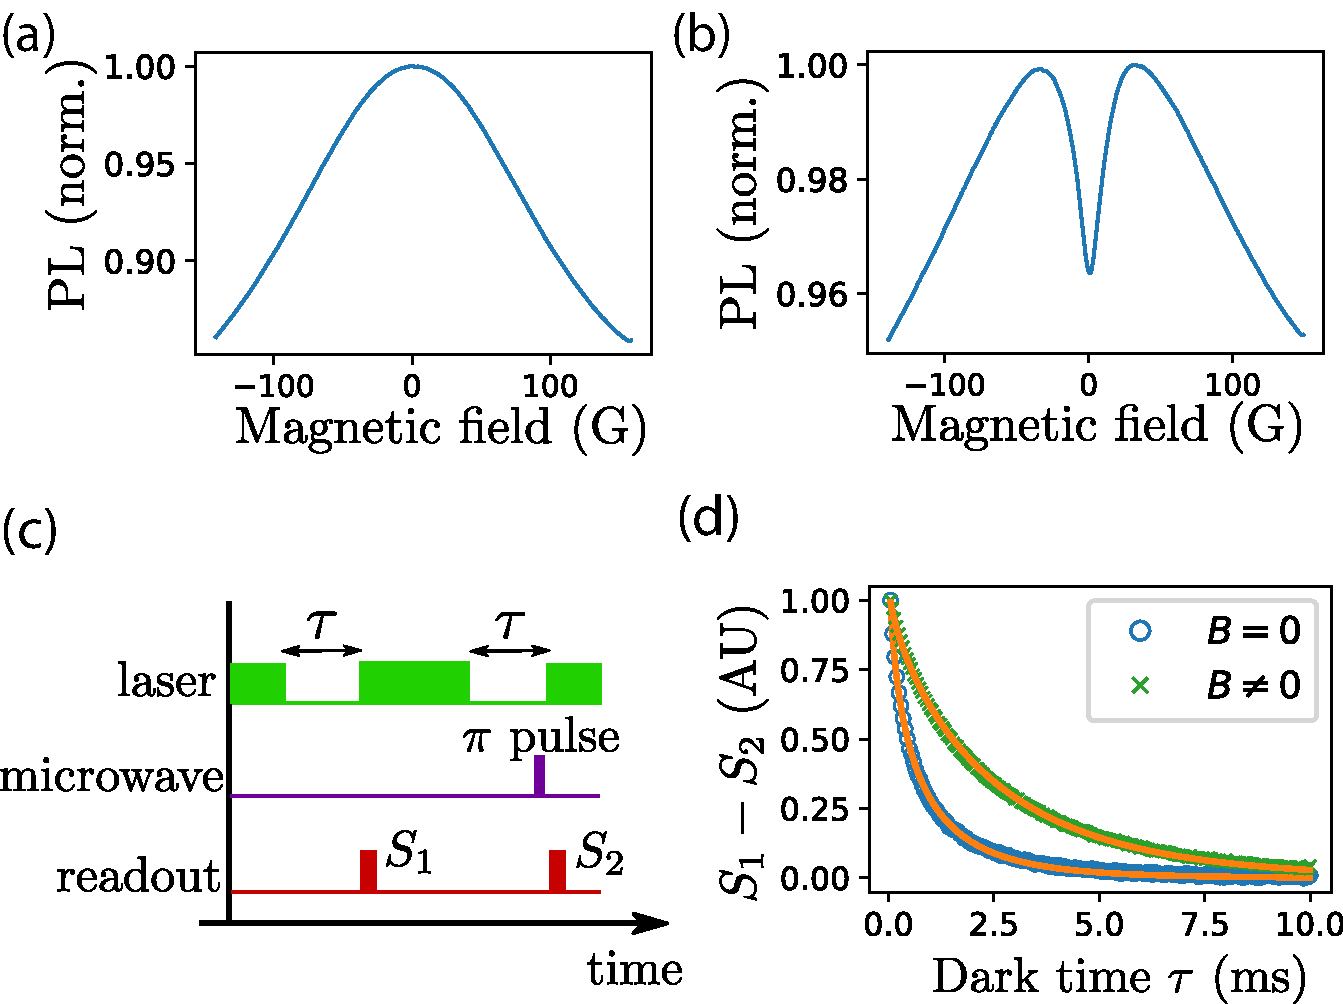
\includegraphics[width=0.45\textwidth]{Figures/fig_T1.pdf}
\caption{a) PL measurement from NV centers ensemble as a function of an external magnetic field applied in an arbitrary direction (a) for the sample CVD-PPB, with [NV$^-$]$\approx 50\ \rm ppb$ (b) for the sample HPHT-150-1, with [NV$^-$]$\approx 3\ \rm ppm$. (c) Sequence used to measure the spin lifetime. (d) Spin relaxation $S_1-S_2$ measured for the dense sample at zero and non-zero magnetic fields. The fitting procedure (orange plain line) is detailed in the main text}
\label{T1}
\end{figure}

\begin{figure*}
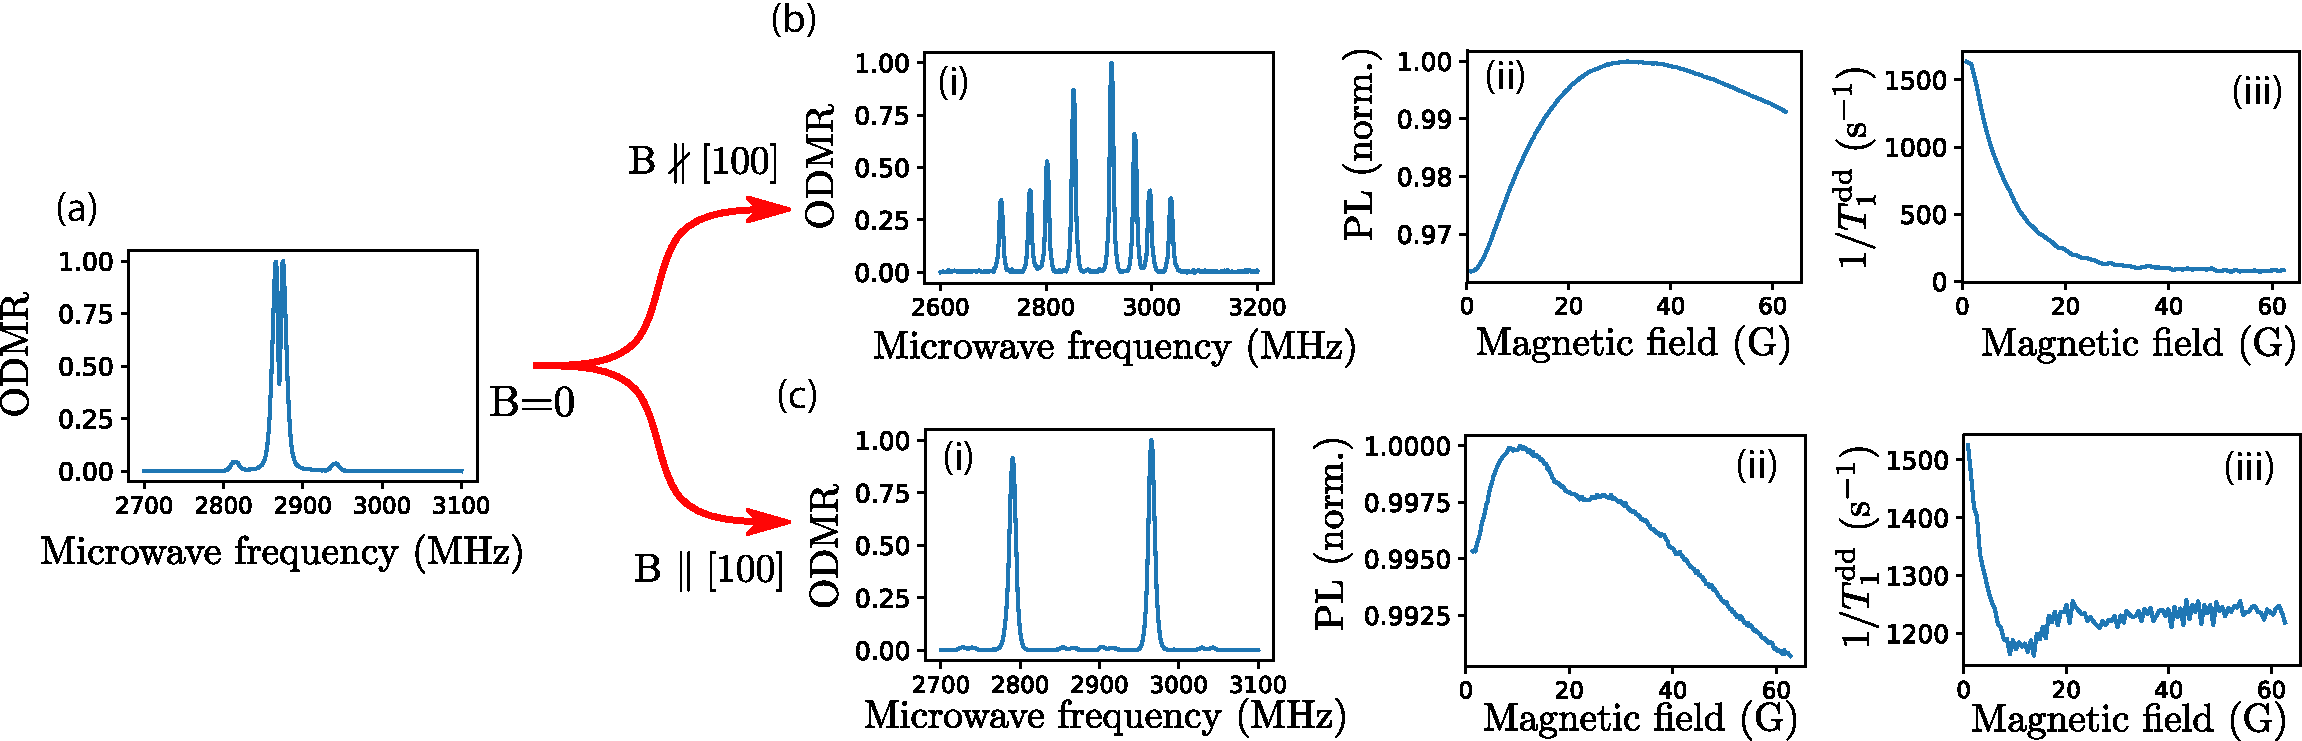
\includegraphics[width=.95\textwidth]{Figures/fig_100_vs_1x1x1x1.pdf}
\caption{(a) ODMR spectrum in zero field. (b)-i) ODMR spectrum for a magnetic field $\approx$ 60 G, misaligned by $\sim  24^\circ$ from the [100] axis. (b)-ii) Normalized PL of the NV$^-$ ensemble as a function of the magnetic field amplitude. (b)-iii) Stretched part of the spin decay $1/T_1^{\rm dd}$ as a function of the magnetic field amplitude. (c)-i), (c)-ii) and (c)-iii) :same measurements but with a magnetic field close to the [100] axis. All the measurements were realized using the sample HPHT-150-1. }
\label{100_VS_1x4}
\end{figure*}

Before analyzing in detail the cause of low-field depolarization, we present $T_1$ measurements realized on HPHT-150-1. Fig. \ref{T1}-c) shows the sequence employed for measuring $T_1^{\rm dd}$. 
It consists in a pump-probe measurement where the spins are first polarized in the $\ket{0}$ state by a green laser, and read-out optically after a variable dark time $\tau$. In highly doped samples, this sequence often results in artifacts, mostly due to charge state transfer in the dark \citep{giri_coupled_2018, giri_selective_2019}. It is therefore convenient to repeat the sequence with an additional $\pi$ pulse right on one of the eight NV spin-resonances before the spin read-out to prepare the remaining $\ket{0}$ polarization into a darker $\ket{+1}$ or $\ket{-1}$ state. By subtracting the result of the two sequences, we select only the spin-dependent part of the signal, with the added benefit of being able to select a specific class of NV centers \citep{jarmola_temperature-_2012, mrozek_longitudinal_2015, choi2017depolarization}. 

Fig. \ref{T1}-d) shows the subtracted signals $S_1-S_2$ when $B\approx 0$ and $B \approx 50\ \rm G$.
The relaxation rate is markedly different in both magnetic field settings, with a much more pronounced depolarization at zero-field.
Notably, the ensemble spin decay curves are not exponential. This was found to be due to inhomogeneities between the spin lifetimes of dipolar coupled NV$^-$ centers \citep{choi2017depolarization}.
We will base our interpretations of the experimental results on the NV-fluctuator model developed in \citep{choi2017depolarization}. This model postulates the existence of very short-lived NV centers - the so-called fluctuators - which, when coupled resonantly to the other NV centers, act as a polarization drain for the spin ensemble. A conclusion of this model is that, for a homogeneous 3D distribution of fluctuators, the dipole-induced relaxation should be a stretched-exponential with a stretch factor $\beta=1/2$. Such a trend was indeed observed when $T_1^{\rm dd} \ll T_1^{\rm ph}$ \cite{choi2017depolarization}. We conducted further measurements to confirm the stretch nature of the dipole-induced decay (see SM sec. IV A), as well as confirming the lifetime-limited model of the fluctuators by measuring the resonance condition between classes of NV centers (see SM sec. IV B).
In our case however, all dense samples used in this paper (detailed in SM sec. II) show $T_1^{\rm dd} \sim T_1^{\rm ph}$, so both decay processes have to be included in the analysis. Fitting the two curves in Fig. 2 d) by the product of a simple and a stretched exponential, we find $T_1^{\rm ph}=3.6$ ms for both curves and $T_1^{\rm dd}= 0.6\ \rm ms$ and $13.0\ \rm ms$ for the $B=0$ and $B=50$G cases respectively. These results thus demonstrates a twenty-fold increase in the dipolar depolarization rate when the B field is turned to zero.
While the fluctuator model developed in \citep{choi2017depolarization} contains some of the explanation for this increase in dipolar depolarization, due to more classes being resonant in zero field than in non-zero field, the model did not include the specificity of the zero magnetic field region, such as the importance of local electric field and the double flip processes. We therefore decided to conducted more in depth experiments in order to characterize these zero field specificities.

Fig. \ref{100_VS_1x4} (a) shows an optically detected magnetic resonance (ODMR) spectrum at zero magnetic field, from the dense ensemble HPHT-150-1.
Fig. \ref{100_VS_1x4} (b)-i) shows an ODMR spectrum from the same sample, but in a magnetic field. The observed lines correspond to the projections of the magnetic fields onto the four classes of NV centers together with the two possible spin transitions $\ket{0}\to\ket{-1}$ and $\ket{0}\to\ket{+1}$. The transitions frequencies of the four different classes can be controlled by changing the amplitude and orientation of the external magnetic field. Fig. \ref{100_VS_1x4} (c)-i) shows an example where all four classes are brought to resonance by placing the magnetic field along the [100] crystalline axis. 
This configuration will be essential to decipher which dipolar relaxation mechanisms play a role at low field. 

Fig. \ref{100_VS_1x4} (b)-ii) show the PL from the NV centers ensemble as a function of the amplitude of a magnetic field aligned as in Fig. \ref{100_VS_1x4} (b)-i). 
Fig. \ref{100_VS_1x4} (b)-iii) shows the stretched exponential spin decay time $T_1^{\rm dd}$ obtained using the sequence shown in Fig. 2-c) in the same range of magnetic field values, in 5 G steps. 
We observe that the 3~\% increase in PL under low magnetic field is indeed correlated with a drop in the spin decay rate from 1.6 kHz to 0.08 kHz, as the magnetic field increases. This result can again be explained by the higher number of resonant spins as the zero magnetic field is reduced, where all four classes are degenerate, as opposed to $\bm B \neq 0$. The half width of the dip ($\approx 10$G) is consistent with a fluctuator model taking into account the change in the spin resonance overlaps as the $B$ field is swept (see SM sec. IV C).
Note that the decrease in PL for $B>40\ \rm G$ is related to state mixing by the transverse magnetic field, so it is not associated with a modification of the spin lifetime. 

Importantly, B field scans along the [100] direction, where the four classes are always resonant, still features an increase of the spin lifetime as the B field increases. Fig. \ref{100_VS_1x4} (c)-ii) and (c)-iii) show the change in the PL and in $1/T_1^{\rm dd}$ as a function of a magnetic field that is aligned in this direction. We can see that there still is an increase in the spin decay rate and a corresponding drop in the PL under low magnetic field values, although considerably reduced. 

The main aim of this paper is to understand the physics governing the contribution to the spin decay in this second scenario. Note that the slight drop in PL and the corresponding bump for $1/T_1^{\rm dd}$ at $B \sim 20$G is related to dipolar interaction with NV centers that have a $^{13}$C as a first neighbor \cite{pellet2021optical}. 

We identify and isolate two additional mechanisms that could explain this effect :local electric fields and double-flip processes. 
 In situations such as the one described in Fig.~\ref{100_VS_1x4} (c)-i), the only relevant terms for depolarisation in $\mathcal{H}^{\rm dd}$ are the flip-flop terms such as $\mel{0,+1}{\mathcal{H}^{\rm dd}}{+1,0}$ where $\mathcal{H}^{\rm dd}$ is the dipole-dipole Hamiltonian detailed in SM sec. V. In zero magnetic field however, we have to take into account two other mechanisms of the dipolar Hamiltonian in consideration.

It was shown in  \cite{mittiga2018imaging} that local electric fields coming from $P_1^+$ or NV$^-$ centers are responsible for the optically detected spin resonance profile at zero magnetic field in dense NV ensembles. Magnetic field noise comes in to second order in zero field. 
We will then consider the following spin Hamiltonian for the electric field dependent NV$^-$ ground state: 
\begin{equation}
\label{NV Hamiltonian}
\mathcal{H}_{\rm elec}= d_\perp \left[ E_x(S_y^2-S_x^2) + E_y(S_xS_y+S_yS_x) \right]
\end{equation}
where $E_{x,y}$ are the projections of local electric fields on the NV axes. 
Under local electric fields with orientations given by the angle $\phi_E={\rm tan}(E_x/E_y)$, the eigenstates of $H_{NV}$ are $\ket{0}$ and $\ket{\pm}=\frac{1}{\sqrt{2}}(\ket{+1}\pm e^{-i\phi_E}\ket{-1})$.
Computing the flip-flop terms $\ket{\pm,0} \bra{0,\pm} $ in the fluctuator model shows that $1/T_1^{\rm dd}$ should be increased at zero field, even after averaging over all possible orientations $\phi_E$ (see SM sec. V).  Another mechanism at stake when considering dipolar interactions with spin-1 systems are double-flip processes. 
These processes correspond to terms like $\ket{+1,0} \bra{0,-1}$ in the dipolar interaction, giving rise to an exchange of two units of spin-angular momentum. These processes can become significant when the states $\ket{m_s=\pm 1}$ are degenerate and are thus likely to explain part of the zero-field dip in Fig. 3-c)-ii). 

\begin{figure}
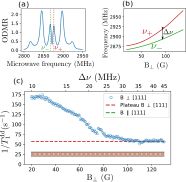
\includegraphics[width=0.45\textwidth]{Figures/fig_transverse_field_V3.pdf}
\caption{(a) Energies of the electronic spin states $\ket{g}$, $\ket{d}$ and $\ket{e}$ under a purely transverse magnetic field $B_\perp$. (b) Blue dashed line :frequency detuning $\Delta \nu$ between the $\ket{e}$ and $\ket{d}$ states. Red plain line :Matching factor $\abs{\bra{e}\ket{+}}^2$ between the states $\ket{e}$ and $\ket{+}$. (c) Measurement of the stretched exponential decay rate $1/T_1^{\rm dd}$ for a single NV class as a function of the amplitude of $B_\perp$. The red dashed line is the value reached for high transverse field. The green dashed line correspond to the value found for the same sample under a longitudinal magnetic field. Error bars are depicted by the shaded pink region. The corresponding detuning between the states $\ket{d}$ and $\ket{e}$ is indicated on the top x-axis. The vertical black dashed line indicates the separation between regions A and B (see main text).}
\label{B_transverse}
\end{figure}

In order to discriminate the role of these two effects in the low-field region, we make use of a purely transverse magnetic field. The transverse B field emulates the effect of the electric field, while turning off the resonance condition for the effectiveness of double-flip processes. Indeed for relatively weak transverse magnetic field, the eigen-basis of the spin Hamiltonian is close to $\ket{0},\ket{+},\ket{-}$. This property has already been used to observe a linear dependence in the electric field for the spin transition frequencies by applying an external transverse magnetic field \cite{dolde2011electric,qiu2022nanoscale}.
Fig.~\ref{B_transverse} (a) shows the energy levels for the three eigenstates of the NV spin Hamiltonian as a function of a purely transverse magnetic field. We will denote these eigenstates in the general case $\ket{g}$, $\ket{d}$ and $\ket{e}$. For weak transverse magnetic field, $\ket{g} \approx \ket{0}$, $\ket{d}=\ket{-}$ and $\ket{e} \approx \ket{+}$. As the magnetic field increases, $\ket{g}$ and $\ket{e}$ starts to become a mixing of $\ket{0}$ and $\ket{+}$ while $\ket{d}$ remains equal to $\ket{-}$.

Crucially, mixing remains even when the associated energy splitting of the $\ket{d}$ and $\ket{e}$ states is large :Fig. \ref{B_transverse}-(b) shows both the splitting between the energy levels of $\ket{d}$ and $\ket{e}$, and the matching factor $\abs{\bra{e}\ket{+}}^2$ characterizing the closeness of the states $\bra{e}$ and $\bra{+}$. We can see that at a field value of $\sim 130$ G, the splitting between the $\ket{d}$ and $\ket{e}$ reaches $\sim 50$ MHz, exceeding the range of the dipole-dipole resonant coupling (see SM sec. IV B). Yet, $\abs{\bra{e}\ket{+}}^2 > 0.98$ meaning that the spin Hamiltonian eigenstates are still roughly in the $\ket{0}, \ket{+}, \ket{-}$ basis. We can therefore decouple the effects of the double-flip processes  $\propto \ket{g,d}\bra{d,e}$, which are no longer resonant when $| \bm B | \geq 100$ G, from the effects of the mixing induced by the transverse electric - or in this case magnetic - field.

Fig. \ref{B_transverse}-(c) shows the measurement of the stretched lifetime $T_1^{\rm dd}$ for a single class of NV centers on sample HPHT-150-2 exposed to a transverse magnetic field between 20 and 130 G.  The detuning $\Delta \nu$ between the two states $\ket{d}$ and $\ket{e}$ was measured through ODMR. Beforehand, we measured a stretched decay $1/T_1^{\rm dd}=25\pm 5\  \rm Hz$ under strong longitudinal magnetic field. This value is indicated by the dashed green line. Two regions can be identified in Fig. \ref{B_transverse}-(c). In  region A, the spin decay rate decreases from 175 Hz to 60 Hz.  We attribute this effect to the loss of effectiveness of the double-flip processes. In region B, $\Delta \nu \geq 30\ \rm MHz$, the decay rate plateaus to $1/T_1^{\rm dd}=57\pm 5\  \rm Hz$, which is about twice as large as the decay rate measured under a longitudinal magnetic field. This plateau can be attributed to the change of eigenstate basis in the presence of transverse magnetic field, which is the same as under low magnetic field, where local transverse electric fields dominates the spin Hamiltonian (see SM sec. I). From these measurements, we conclude that the effect of the double-flip processes is about 5 times more important than the effect of the electric field in the depolarization rate.

Based on an extension of the fluctuator model developed in SM sec. V, we predict an overall increase by a factor of $\sim 4$ of the dipole-dipole induced decay rate in the non-magnetic basis $\ket{0}, \ket{+}, \ket{-}$ compared to the magnetic basis $\ket{0}, \ket{+1}, \ket{-1}$. While the measured increase is smaller than the predicted one, the measurements agrees with the theoretical increase in the flip-flop rate in the $\ket{+/-}$ basis compared to the $\ket{\pm 1}$ basis. Similarly, we compute the predicted decay rate when $\bm B \parallel \left[100\right]$ case compared when $\bm B = 0$, and find a theoretical increase of $\sim 20\%$ when $\bm B = 0$ due to the mixing by the local electric field. This, along with the double-flip processes explains the behavior observed in Fig. \ref{100_VS_1x4} (c)-ii) and (c)-iii).

\begin{figure}
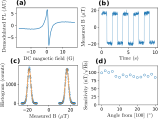
\includegraphics[width=0.45\textwidth]{Figures/fig_magneto}
\caption{Low-field magnetometry protocol. (a) Demodulated PL as a function of an externally applied magnetic field with an additional oscillatory magnetic field. (b) Measured magnetic field when alternating a small external magnetic field offset. (c) Histogram of the measurement in Fig. (b) fitted by gaussians of standard deviation $\sigma=1.5\ \mu \rm T$. (d) Measured sensitivity as function of the angle between the external magnetic field and the [100] crystalline axis.}
\label{magneto}
\end{figure}


Our observations have important implications for magnetometry with NV ensembles.
DC microwave-free magnetometry has already been performed using either NV-NV cross-relaxations \citep{akhmedzhanov_microwave-free_2017,akhmedzhanov_magnetometry_2019} or level anti-crossing \citep{Wickenbrock, zheng2017level, zheng_microwave-free_2020}. Here we propose to perform a similar protocol, but using the spin depolarization at zero-field as proposed in \cite{filimonenko2018weak, filimonenko2022manifestation}. The main advantage compared to previously employed protocols is that the sensitivity does not depend crucially on crystalline orientation, making this protocol applicable with diamond powders or polycrystalline samples. Another sizable advantage is that this measurement is that it is insensitive to thermal variations. In order to optimize signal-to-noise ratio, we use a lock-in detection and add a magnetic field modulation at $\sim 1\ \rm kHz$ with an amplitude $\sim 10\ \rm G$ through the same electromagnet. Fig. \ref{magneto}-(a) shows the demodulated PL as a DC magnetic field is scanned in an arbitrary direction. The sample used here is HPHT-15-1, the laser power $\sim 1\ \rm mW$ and the collected PL is $\sim 1\ \mu\rm W$.  We can see a sharp linear slope in low field $\abs{B} < 5\ \rm G$. Once calibrated, in this case with ODMR, the slope provides a 1D magnetic field measurement, which could be extended to 3D with a set of 3 coils or 3 electromagnets, as in \cite{zheng_microwave-free_2020}. In order to assess the sensitivity of the measurement, we alternate a small DC field of $\approx 40\ \mu\rm{T}$ every few seconds and take a histogram of the measured fields (46.000 counts in 46 s), as shown in Fig. \ref{magneto} (b) and (c). The histogram is well fitted by gaussians of standard deviation $\sigma=1.5\ \mu \rm T$. The measurement was performed here with an output low-pass filter of time constant $\tau=3\ \rm ms$, which gives us a DC sensitivity $\eta=\sigma \sqrt{\tau}=82\ \rm{nT}/\sqrt{\rm Hz}$. Normalized to the volume, this gives $\eta/\sqrt{V}\approx 4.7 \ \mu \rm{T}/\mu m^{3/2}/\sqrt{\rm Hz}$. This measurement is consistent with the experimentally found $\sim 5\ \mu \rm{T}/\sqrt{\rm Hz}$ sensitivity obtained with sample HPHT-1-1 (see samples details in SM sec. II).

We now evaluate the relative role of the three causes of spin depolarization that assist the operation of the magnetometer, namely the splitting of the NV classes, the local electric field and the double-flip processes. In order to do so, we measure the magnetometer sensitivity while changing the angle of the magnetic field.  The results are shown in Fig. \ref{magneto} (d). We can see a $\sim$ 10\% declining sensitivity as we leave the [100] region, but overall the sensitivity remains relatively invariant. 
When $\bm B$ is aligned with the [100] crystalline axis, only the double flips and the electric field cause a depolarization, whereas in every other orientation the three effects are at play.
The double-flips and electric field effects are thus the dominant factors in the sensitivity of this protocol. While it may seem surprising that the effects with a lower contribution to the PL contrast have a higher effect on this PL-based protocol, what matters here is not the absolute contrast but the slope of the change of contrast with respect to the magnetic field. The latter is in fact larger for the local electric field and double flips processes than for the process involving only flip-flops. 
It should be noted that this observation is sample dependent, and that other samples, including from the same batch, have shown a higher orientation dependence, corresponding to a lower contribution from the electric field and double-flip processes.

As a conclusion, we identified three mechanisms causing extra spin depolarization in zero field for dense ensemble of NV$^-$ centers, all related to an increase in the dipole-dipole induced CR between the spins of NV centers. The lift in degeneracy of the spin state of different NV classes was found to be the main cause of zero-field depolarization, followed by double-flip processes and then the electric field induced mixing. We have employed CR for microwave and orientation-free DC-magnetometry and demonstrated a sensitivity below $100\ \rm{nm}/\sqrt{\rm Hz}$ for a single $15\ \mu \rm m$ commercially available diamond and show that that double-flips and electric field play an important role.
Our studies will be important for microwave based low field magnetometry \cite{Vetter_LFM, WangRB}. 
Besides magnetometry, our work offers prospects for understanding many body phenomena with strongly coupled spins under purely transverse as well as small magnetic fields. 

\section*{acknowledgements}

We would like to acknowledge support from Alexandre Tallaire and Jocelyn Achard as well as 
SIRTEQ for funding.

%\bibliographystyle{unsrtnat}
%\bibliographystyle{apsrev4-2}
%\bibliography{CR}{}

%apsrev4-2.bst 2019-01-14 (MD) hand-edited version of apsrev4-1.bst
%Control: key (0)
%Control: author (72) initials jnrlst
%Control: editor formatted (1) identically to author
%Control: production of article title (-1) disabled
%Control: page (0) single
%Control: year (1) truncated
%Control: production of eprint (0) enabled
\begin{thebibliography}{41}%
\makeatletter
\providecommand \@ifxundefined [1]{%
 \@ifx{#1\undefined}
}%
\providecommand \@ifnum [1]{%
 \ifnum #1\expandafter \@firstoftwo
 \else \expandafter \@secondoftwo
 \fi
}%
\providecommand \@ifx [1]{%
 \ifx #1\expandafter \@firstoftwo
 \else \expandafter \@secondoftwo
 \fi
}%
\providecommand \natexlab [1]{#1}%
\providecommand \enquote  [1]{``#1''}%
\providecommand \bibnamefont  [1]{#1}%
\providecommand \bibfnamefont [1]{#1}%
\providecommand \citenamefont [1]{#1}%
\providecommand \href@noop [0]{\@secondoftwo}%
\providecommand \href [0]{\begingroup \@sanitize@url \@href}%
\providecommand \@href[1]{\@@startlink{#1}\@@href}%
\providecommand \@@href[1]{\endgroup#1\@@endlink}%
\providecommand \@sanitize@url [0]{\catcode `\\12\catcode `\$12\catcode
  `\&12\catcode `\#12\catcode `\^12\catcode `\_12\catcode `\%12\relax}%
\providecommand \@@startlink[1]{}%
\providecommand \@@endlink[0]{}%
\providecommand \url  [0]{\begingroup\@sanitize@url \@url }%
\providecommand \@url [1]{\endgroup\@href {#1}{\urlprefix }}%
\providecommand \urlprefix  [0]{URL }%
\providecommand \Eprint [0]{\href }%
\providecommand \doibase [0]{https://doi.org/}%
\providecommand \selectlanguage [0]{\@gobble}%
\providecommand \bibinfo  [0]{\@secondoftwo}%
\providecommand \bibfield  [0]{\@secondoftwo}%
\providecommand \translation [1]{[#1]}%
\providecommand \BibitemOpen [0]{}%
\providecommand \bibitemStop [0]{}%
\providecommand \bibitemNoStop [0]{.\EOS\space}%
\providecommand \EOS [0]{\spacefactor3000\relax}%
\providecommand \BibitemShut  [1]{\csname bibitem#1\endcsname}%
\let\auto@bib@innerbib\@empty
%</preamble>
\bibitem [{\citenamefont {Doherty}\ \emph {et~al.}(2013)\citenamefont
  {Doherty}, \citenamefont {Manson}, \citenamefont {Delaney}, \citenamefont
  {Jelezko}, \citenamefont {Wrachtrup},\ and\ \citenamefont
  {Hollenberg}}]{DOHERTY20131}%
  \BibitemOpen
  \bibfield  {author} {\bibinfo {author} {\bibfnamefont {M.~W.}\ \bibnamefont
  {Doherty}}, \bibinfo {author} {\bibfnamefont {N.~B.}\ \bibnamefont {Manson}},
  \bibinfo {author} {\bibfnamefont {P.}~\bibnamefont {Delaney}}, \bibinfo
  {author} {\bibfnamefont {F.}~\bibnamefont {Jelezko}}, \bibinfo {author}
  {\bibfnamefont {J.}~\bibnamefont {Wrachtrup}},\ and\ \bibinfo {author}
  {\bibfnamefont {L.~C.}\ \bibnamefont {Hollenberg}},\ }\href
  {https://doi.org/https://doi.org/10.1016/j.physrep.2013.02.001} {\bibfield
  {journal} {\bibinfo  {journal} {Physics Reports}\ }\textbf {\bibinfo {volume}
  {528}},\ \bibinfo {pages} {1 } (\bibinfo {year} {2013})},\ \bibinfo {note}
  {the nitrogen-vacancy colour centre in diamond}\BibitemShut {NoStop}%
\bibitem [{\citenamefont {Acosta}\ \emph {et~al.}(2009)\citenamefont {Acosta},
  \citenamefont {Bauch}, \citenamefont {Ledbetter}, \citenamefont {Santori},
  \citenamefont {Fu}, \citenamefont {Barclay}, \citenamefont {Beausoleil},
  \citenamefont {Linget}, \citenamefont {Roch}, \citenamefont {Treussart},
  \citenamefont {Chemerisov}, \citenamefont {Gawlik},\ and\ \citenamefont
  {Budker}}]{Acosta}%
  \BibitemOpen
  \bibfield  {author} {\bibinfo {author} {\bibfnamefont {V.~M.}\ \bibnamefont
  {Acosta}}, \bibinfo {author} {\bibfnamefont {E.}~\bibnamefont {Bauch}},
  \bibinfo {author} {\bibfnamefont {M.~P.}\ \bibnamefont {Ledbetter}}, \bibinfo
  {author} {\bibfnamefont {C.}~\bibnamefont {Santori}}, \bibinfo {author}
  {\bibfnamefont {K.-M.~C.}\ \bibnamefont {Fu}}, \bibinfo {author}
  {\bibfnamefont {P.~E.}\ \bibnamefont {Barclay}}, \bibinfo {author}
  {\bibfnamefont {R.~G.}\ \bibnamefont {Beausoleil}}, \bibinfo {author}
  {\bibfnamefont {H.}~\bibnamefont {Linget}}, \bibinfo {author} {\bibfnamefont
  {J.~F.}\ \bibnamefont {Roch}}, \bibinfo {author} {\bibfnamefont
  {F.}~\bibnamefont {Treussart}}, \bibinfo {author} {\bibfnamefont
  {S.}~\bibnamefont {Chemerisov}}, \bibinfo {author} {\bibfnamefont
  {W.}~\bibnamefont {Gawlik}},\ and\ \bibinfo {author} {\bibfnamefont
  {D.}~\bibnamefont {Budker}},\ }\href
  {https://doi.org/10.1103/PhysRevB.80.115202} {\bibfield  {journal} {\bibinfo
  {journal} {Phys. Rev. B}\ }\textbf {\bibinfo {volume} {80}},\ \bibinfo
  {pages} {115202} (\bibinfo {year} {2009})}\BibitemShut {NoStop}%
\bibitem [{\citenamefont {Tallaire}\ \emph {et~al.}(2020)\citenamefont
  {Tallaire}, \citenamefont {Brinza}, \citenamefont {Huillery}, \citenamefont
  {Delord}, \citenamefont {Pellet-Mary}, \citenamefont {Staacke}, \citenamefont
  {Abel}, \citenamefont {Pezzagna}, \citenamefont {Meijer}, \citenamefont
  {Touati}, \citenamefont {Binet}, \citenamefont {Ferrier}, \citenamefont
  {Goldner}, \citenamefont {Hetet},\ and\ \citenamefont
  {Achard}}]{TALLAIRE2020421}%
  \BibitemOpen
  \bibfield  {author} {\bibinfo {author} {\bibfnamefont {A.}~\bibnamefont
  {Tallaire}}, \bibinfo {author} {\bibfnamefont {O.}~\bibnamefont {Brinza}},
  \bibinfo {author} {\bibfnamefont {P.}~\bibnamefont {Huillery}}, \bibinfo
  {author} {\bibfnamefont {T.}~\bibnamefont {Delord}}, \bibinfo {author}
  {\bibfnamefont {C.}~\bibnamefont {Pellet-Mary}}, \bibinfo {author}
  {\bibfnamefont {R.}~\bibnamefont {Staacke}}, \bibinfo {author} {\bibfnamefont
  {B.}~\bibnamefont {Abel}}, \bibinfo {author} {\bibfnamefont {S.}~\bibnamefont
  {Pezzagna}}, \bibinfo {author} {\bibfnamefont {J.}~\bibnamefont {Meijer}},
  \bibinfo {author} {\bibfnamefont {N.}~\bibnamefont {Touati}}, \bibinfo
  {author} {\bibfnamefont {L.}~\bibnamefont {Binet}}, \bibinfo {author}
  {\bibfnamefont {A.}~\bibnamefont {Ferrier}}, \bibinfo {author} {\bibfnamefont
  {P.}~\bibnamefont {Goldner}}, \bibinfo {author} {\bibfnamefont
  {G.}~\bibnamefont {Hetet}},\ and\ \bibinfo {author} {\bibfnamefont
  {J.}~\bibnamefont {Achard}},\ }\href
  {https://doi.org/https://doi.org/10.1016/j.carbon.2020.08.048} {\bibfield
  {journal} {\bibinfo  {journal} {Carbon}\ }\textbf {\bibinfo {volume} {170}},\
  \bibinfo {pages} {421 } (\bibinfo {year} {2020})}\BibitemShut {NoStop}%
\bibitem [{\citenamefont {Edmonds}\ \emph {et~al.}(2021)\citenamefont
  {Edmonds}, \citenamefont {Hart}, \citenamefont {Turner}, \citenamefont
  {Colard}, \citenamefont {Schloss}, \citenamefont {Olsson}, \citenamefont
  {Trubko}, \citenamefont {Markham}, \citenamefont {Rathmill}, \citenamefont
  {Horne-Smith} \emph {et~al.}}]{edmonds2021characterisation}%
  \BibitemOpen
  \bibfield  {author} {\bibinfo {author} {\bibfnamefont {A.~M.}\ \bibnamefont
  {Edmonds}}, \bibinfo {author} {\bibfnamefont {C.~A.}\ \bibnamefont {Hart}},
  \bibinfo {author} {\bibfnamefont {M.~J.}\ \bibnamefont {Turner}}, \bibinfo
  {author} {\bibfnamefont {P.-O.}\ \bibnamefont {Colard}}, \bibinfo {author}
  {\bibfnamefont {J.~M.}\ \bibnamefont {Schloss}}, \bibinfo {author}
  {\bibfnamefont {K.~S.}\ \bibnamefont {Olsson}}, \bibinfo {author}
  {\bibfnamefont {R.}~\bibnamefont {Trubko}}, \bibinfo {author} {\bibfnamefont
  {M.~L.}\ \bibnamefont {Markham}}, \bibinfo {author} {\bibfnamefont
  {A.}~\bibnamefont {Rathmill}}, \bibinfo {author} {\bibfnamefont
  {B.}~\bibnamefont {Horne-Smith}}, \emph {et~al.},\ }\href@noop {} {\bibfield
  {journal} {\bibinfo  {journal} {Materials for Quantum Technology}\ }\textbf
  {\bibinfo {volume} {1}},\ \bibinfo {pages} {025001} (\bibinfo {year}
  {2021})}\BibitemShut {NoStop}%
\bibitem [{\citenamefont {Chatzidrosos}\ \emph {et~al.}(2021)\citenamefont
  {Chatzidrosos}, \citenamefont {Rebeirro}, \citenamefont {Zheng},
  \citenamefont {Omar}, \citenamefont {Brenneis}, \citenamefont {St{\"u}rner},
  \citenamefont {Fuchs}, \citenamefont {Buck}, \citenamefont {R{\"o}lver},
  \citenamefont {Schneemann} \emph {et~al.}}]{chatzidrosos2021fiberized}%
  \BibitemOpen
  \bibfield  {author} {\bibinfo {author} {\bibfnamefont {G.}~\bibnamefont
  {Chatzidrosos}}, \bibinfo {author} {\bibfnamefont {J.~S.}\ \bibnamefont
  {Rebeirro}}, \bibinfo {author} {\bibfnamefont {H.}~\bibnamefont {Zheng}},
  \bibinfo {author} {\bibfnamefont {M.}~\bibnamefont {Omar}}, \bibinfo {author}
  {\bibfnamefont {A.}~\bibnamefont {Brenneis}}, \bibinfo {author}
  {\bibfnamefont {F.~M.}\ \bibnamefont {St{\"u}rner}}, \bibinfo {author}
  {\bibfnamefont {T.}~\bibnamefont {Fuchs}}, \bibinfo {author} {\bibfnamefont
  {T.}~\bibnamefont {Buck}}, \bibinfo {author} {\bibfnamefont {R.}~\bibnamefont
  {R{\"o}lver}}, \bibinfo {author} {\bibfnamefont {T.}~\bibnamefont
  {Schneemann}}, \emph {et~al.},\ }\href@noop {} {\bibfield  {journal}
  {\bibinfo  {journal} {Frontiers in Photonics}\ ,\ \bibinfo {pages} {4}}
  (\bibinfo {year} {2021})}\BibitemShut {NoStop}%
\bibitem [{\citenamefont {Kucsko}\ \emph {et~al.}(2018)\citenamefont {Kucsko},
  \citenamefont {Choi}, \citenamefont {Choi}, \citenamefont {Maurer},
  \citenamefont {Zhou}, \citenamefont {Landig}, \citenamefont {Sumiya},
  \citenamefont {Onoda}, \citenamefont {Isoya}, \citenamefont {Jelezko} \emph
  {et~al.}}]{kucsko2018critical}%
  \BibitemOpen
  \bibfield  {author} {\bibinfo {author} {\bibfnamefont {G.}~\bibnamefont
  {Kucsko}}, \bibinfo {author} {\bibfnamefont {S.}~\bibnamefont {Choi}},
  \bibinfo {author} {\bibfnamefont {J.}~\bibnamefont {Choi}}, \bibinfo {author}
  {\bibfnamefont {P.~C.}\ \bibnamefont {Maurer}}, \bibinfo {author}
  {\bibfnamefont {H.}~\bibnamefont {Zhou}}, \bibinfo {author} {\bibfnamefont
  {R.}~\bibnamefont {Landig}}, \bibinfo {author} {\bibfnamefont
  {H.}~\bibnamefont {Sumiya}}, \bibinfo {author} {\bibfnamefont
  {S.}~\bibnamefont {Onoda}}, \bibinfo {author} {\bibfnamefont
  {J.}~\bibnamefont {Isoya}}, \bibinfo {author} {\bibfnamefont
  {F.}~\bibnamefont {Jelezko}}, \emph {et~al.},\ }\href@noop {} {\bibfield
  {journal} {\bibinfo  {journal} {Physical review letters}\ }\textbf {\bibinfo
  {volume} {121}},\ \bibinfo {pages} {023601} (\bibinfo {year}
  {2018})}\BibitemShut {NoStop}%
\bibitem [{\citenamefont {Choi}\ \emph
  {et~al.}(2017{\natexlab{a}})\citenamefont {Choi}, \citenamefont {Choi},
  \citenamefont {Landig}, \citenamefont {Kucsko}, \citenamefont {Zhou},
  \citenamefont {Isoya}, \citenamefont {Jelezko}, \citenamefont {Onoda},
  \citenamefont {Sumiya}, \citenamefont {Khemani}, \citenamefont {von
  Keyserlingk}, \citenamefont {Yao}, \citenamefont {Demler},\ and\
  \citenamefont {Lukin}}]{ChoiNat}%
  \BibitemOpen
  \bibfield  {author} {\bibinfo {author} {\bibfnamefont {S.}~\bibnamefont
  {Choi}}, \bibinfo {author} {\bibfnamefont {J.}~\bibnamefont {Choi}}, \bibinfo
  {author} {\bibfnamefont {R.}~\bibnamefont {Landig}}, \bibinfo {author}
  {\bibfnamefont {G.}~\bibnamefont {Kucsko}}, \bibinfo {author} {\bibfnamefont
  {H.}~\bibnamefont {Zhou}}, \bibinfo {author} {\bibfnamefont {J.}~\bibnamefont
  {Isoya}}, \bibinfo {author} {\bibfnamefont {F.}~\bibnamefont {Jelezko}},
  \bibinfo {author} {\bibfnamefont {S.}~\bibnamefont {Onoda}}, \bibinfo
  {author} {\bibfnamefont {H.}~\bibnamefont {Sumiya}}, \bibinfo {author}
  {\bibfnamefont {V.}~\bibnamefont {Khemani}}, \bibinfo {author} {\bibfnamefont
  {C.}~\bibnamefont {von Keyserlingk}}, \bibinfo {author} {\bibfnamefont
  {N.~Y.}\ \bibnamefont {Yao}}, \bibinfo {author} {\bibfnamefont
  {E.}~\bibnamefont {Demler}},\ and\ \bibinfo {author} {\bibfnamefont {M.~D.}\
  \bibnamefont {Lukin}},\ }\href@noop {} {\bibfield  {journal} {\bibinfo
  {journal} {Nature}\ }\textbf {\bibinfo {volume} {543}},\ \bibinfo {pages}
  {221} (\bibinfo {year} {2017}{\natexlab{a}})}\BibitemShut {NoStop}%
\bibitem [{\citenamefont {Zu}\ \emph {et~al.}(2021)\citenamefont {Zu},
  \citenamefont {Machado}, \citenamefont {Ye}, \citenamefont {Choi},
  \citenamefont {Kobrin}, \citenamefont {Mittiga}, \citenamefont {Hsieh},
  \citenamefont {Bhattacharyya}, \citenamefont {Markham}, \citenamefont
  {Twitchen}, \citenamefont {Jarmola}, \citenamefont {Budker}, \citenamefont
  {Laumann}, \citenamefont {Moore},\ and\ \citenamefont {Yao}}]{ZuYao}%
  \BibitemOpen
  \bibfield  {author} {\bibinfo {author} {\bibfnamefont {C.}~\bibnamefont
  {Zu}}, \bibinfo {author} {\bibfnamefont {F.}~\bibnamefont {Machado}},
  \bibinfo {author} {\bibfnamefont {B.}~\bibnamefont {Ye}}, \bibinfo {author}
  {\bibfnamefont {S.}~\bibnamefont {Choi}}, \bibinfo {author} {\bibfnamefont
  {B.}~\bibnamefont {Kobrin}}, \bibinfo {author} {\bibfnamefont
  {T.}~\bibnamefont {Mittiga}}, \bibinfo {author} {\bibfnamefont
  {S.}~\bibnamefont {Hsieh}}, \bibinfo {author} {\bibfnamefont
  {P.}~\bibnamefont {Bhattacharyya}}, \bibinfo {author} {\bibfnamefont
  {M.}~\bibnamefont {Markham}}, \bibinfo {author} {\bibfnamefont
  {D.}~\bibnamefont {Twitchen}}, \bibinfo {author} {\bibfnamefont
  {A.}~\bibnamefont {Jarmola}}, \bibinfo {author} {\bibfnamefont
  {D.}~\bibnamefont {Budker}}, \bibinfo {author} {\bibfnamefont {C.~R.}\
  \bibnamefont {Laumann}}, \bibinfo {author} {\bibfnamefont {J.~E.}\
  \bibnamefont {Moore}},\ and\ \bibinfo {author} {\bibfnamefont {N.~Y.}\
  \bibnamefont {Yao}},\ }\href@noop {} {\bibfield  {journal} {\bibinfo
  {journal} {Nature}\ }\textbf {\bibinfo {volume} {597}},\ \bibinfo {pages}
  {45} (\bibinfo {year} {2021})}\BibitemShut {NoStop}%
\bibitem [{\citenamefont {Choi}\ \emph
  {et~al.}(2017{\natexlab{b}})\citenamefont {Choi}, \citenamefont {Choi},
  \citenamefont {Landig}, \citenamefont {Kucsko}, \citenamefont {Zhou},
  \citenamefont {Isoya}, \citenamefont {Jelezko}, \citenamefont {Onoda},
  \citenamefont {Sumiya}, \citenamefont {Khemani}, \citenamefont {von
  Keyserlingk}, \citenamefont {Yao}, \citenamefont {Demler},\ and\
  \citenamefont {Lukin}}]{choi_observation_2017}%
  \BibitemOpen
  \bibfield  {author} {\bibinfo {author} {\bibfnamefont {S.}~\bibnamefont
  {Choi}}, \bibinfo {author} {\bibfnamefont {J.}~\bibnamefont {Choi}}, \bibinfo
  {author} {\bibfnamefont {R.}~\bibnamefont {Landig}}, \bibinfo {author}
  {\bibfnamefont {G.}~\bibnamefont {Kucsko}}, \bibinfo {author} {\bibfnamefont
  {H.}~\bibnamefont {Zhou}}, \bibinfo {author} {\bibfnamefont {J.}~\bibnamefont
  {Isoya}}, \bibinfo {author} {\bibfnamefont {F.}~\bibnamefont {Jelezko}},
  \bibinfo {author} {\bibfnamefont {S.}~\bibnamefont {Onoda}}, \bibinfo
  {author} {\bibfnamefont {H.}~\bibnamefont {Sumiya}}, \bibinfo {author}
  {\bibfnamefont {V.}~\bibnamefont {Khemani}}, \bibinfo {author} {\bibfnamefont
  {C.}~\bibnamefont {von Keyserlingk}}, \bibinfo {author} {\bibfnamefont
  {N.~Y.}\ \bibnamefont {Yao}}, \bibinfo {author} {\bibfnamefont
  {E.}~\bibnamefont {Demler}},\ and\ \bibinfo {author} {\bibfnamefont {M.~D.}\
  \bibnamefont {Lukin}},\ }\href {https://doi.org/10.1038/nature21426}
  {\bibfield  {journal} {\bibinfo  {journal} {Nature}\ }\textbf {\bibinfo
  {volume} {543}},\ \bibinfo {pages} {221} (\bibinfo {year}
  {2017}{\natexlab{b}})},\ \bibinfo {note} {number: 7644 Publisher: Nature
  Publishing Group}\BibitemShut {NoStop}%
\bibitem [{\citenamefont {Zhou}\ \emph {et~al.}(2020)\citenamefont {Zhou},
  \citenamefont {Choi}, \citenamefont {Choi}, \citenamefont {Landig},
  \citenamefont {Douglas}, \citenamefont {Isoya}, \citenamefont {Jelezko},
  \citenamefont {Onoda}, \citenamefont {Sumiya}, \citenamefont {Cappellaro}
  \emph {et~al.}}]{zhou2020quantum}%
  \BibitemOpen
  \bibfield  {author} {\bibinfo {author} {\bibfnamefont {H.}~\bibnamefont
  {Zhou}}, \bibinfo {author} {\bibfnamefont {J.}~\bibnamefont {Choi}}, \bibinfo
  {author} {\bibfnamefont {S.}~\bibnamefont {Choi}}, \bibinfo {author}
  {\bibfnamefont {R.}~\bibnamefont {Landig}}, \bibinfo {author} {\bibfnamefont
  {A.~M.}\ \bibnamefont {Douglas}}, \bibinfo {author} {\bibfnamefont
  {J.}~\bibnamefont {Isoya}}, \bibinfo {author} {\bibfnamefont
  {F.}~\bibnamefont {Jelezko}}, \bibinfo {author} {\bibfnamefont
  {S.}~\bibnamefont {Onoda}}, \bibinfo {author} {\bibfnamefont
  {H.}~\bibnamefont {Sumiya}}, \bibinfo {author} {\bibfnamefont
  {P.}~\bibnamefont {Cappellaro}}, \emph {et~al.},\ }\href@noop {} {\bibfield
  {journal} {\bibinfo  {journal} {Physical review X}\ }\textbf {\bibinfo
  {volume} {10}},\ \bibinfo {pages} {031003} (\bibinfo {year}
  {2020})}\BibitemShut {NoStop}%
\bibitem [{\citenamefont {Akhmedzhanov}\ \emph {et~al.}(2017)\citenamefont
  {Akhmedzhanov}, \citenamefont {Gushchin}, \citenamefont {Nizov},
  \citenamefont {Nizov}, \citenamefont {Sobgayda}, \citenamefont {Zelensky},\
  and\ \citenamefont {Hemmer}}]{akhmedzhanov_microwave-free_2017}%
  \BibitemOpen
  \bibfield  {author} {\bibinfo {author} {\bibfnamefont {R.}~\bibnamefont
  {Akhmedzhanov}}, \bibinfo {author} {\bibfnamefont {L.}~\bibnamefont
  {Gushchin}}, \bibinfo {author} {\bibfnamefont {N.}~\bibnamefont {Nizov}},
  \bibinfo {author} {\bibfnamefont {V.}~\bibnamefont {Nizov}}, \bibinfo
  {author} {\bibfnamefont {D.}~\bibnamefont {Sobgayda}}, \bibinfo {author}
  {\bibfnamefont {I.}~\bibnamefont {Zelensky}},\ and\ \bibinfo {author}
  {\bibfnamefont {P.}~\bibnamefont {Hemmer}},\ }\href
  {https://doi.org/10.1103/PhysRevA.96.013806} {\bibfield  {journal} {\bibinfo
  {journal} {Phys. Rev. A}\ }\textbf {\bibinfo {volume} {96}},\ \bibinfo
  {pages} {013806} (\bibinfo {year} {2017})},\ \bibinfo {note} {number:
  1}\BibitemShut {NoStop}%
\bibitem [{\citenamefont {Akhmedzhanov}\ \emph {et~al.}(2019)\citenamefont
  {Akhmedzhanov}, \citenamefont {Gushchin}, \citenamefont {Nizov},
  \citenamefont {Nizov}, \citenamefont {Sobgayda}, \citenamefont {Zelensky},\
  and\ \citenamefont {Hemmer}}]{akhmedzhanov_magnetometry_2019}%
  \BibitemOpen
  \bibfield  {author} {\bibinfo {author} {\bibfnamefont {R.}~\bibnamefont
  {Akhmedzhanov}}, \bibinfo {author} {\bibfnamefont {L.}~\bibnamefont
  {Gushchin}}, \bibinfo {author} {\bibfnamefont {N.}~\bibnamefont {Nizov}},
  \bibinfo {author} {\bibfnamefont {V.}~\bibnamefont {Nizov}}, \bibinfo
  {author} {\bibfnamefont {D.}~\bibnamefont {Sobgayda}}, \bibinfo {author}
  {\bibfnamefont {I.}~\bibnamefont {Zelensky}},\ and\ \bibinfo {author}
  {\bibfnamefont {P.}~\bibnamefont {Hemmer}},\ }\href
  {https://doi.org/10.1103/PhysRevA.100.043844} {\bibfield  {journal} {\bibinfo
   {journal} {Phys. Rev. A}\ }\textbf {\bibinfo {volume} {100}},\ \bibinfo
  {pages} {043844} (\bibinfo {year} {2019})},\ \bibinfo {note} {number:
  4}\BibitemShut {NoStop}%
\bibitem [{\citenamefont {Wolf}\ \emph {et~al.}(2015)\citenamefont {Wolf},
  \citenamefont {Neumann}, \citenamefont {Nakamura}, \citenamefont {Sumiya},
  \citenamefont {Ohshima}, \citenamefont {Isoya},\ and\ \citenamefont
  {Wrachtrup}}]{Wolf}%
  \BibitemOpen
  \bibfield  {author} {\bibinfo {author} {\bibfnamefont {T.}~\bibnamefont
  {Wolf}}, \bibinfo {author} {\bibfnamefont {P.}~\bibnamefont {Neumann}},
  \bibinfo {author} {\bibfnamefont {K.}~\bibnamefont {Nakamura}}, \bibinfo
  {author} {\bibfnamefont {H.}~\bibnamefont {Sumiya}}, \bibinfo {author}
  {\bibfnamefont {T.}~\bibnamefont {Ohshima}}, \bibinfo {author} {\bibfnamefont
  {J.}~\bibnamefont {Isoya}},\ and\ \bibinfo {author} {\bibfnamefont
  {J.}~\bibnamefont {Wrachtrup}},\ }\href
  {https://doi.org/10.1103/PhysRevX.5.041001} {\bibfield  {journal} {\bibinfo
  {journal} {Phys. Rev. X}\ }\textbf {\bibinfo {volume} {5}},\ \bibinfo {pages}
  {041001} (\bibinfo {year} {2015})}\BibitemShut {NoStop}%
\bibitem [{\citenamefont {Stürner}\ \emph {et~al.}(2021)\citenamefont
  {Stürner}, \citenamefont {Brenneis}, \citenamefont {Buck}, \citenamefont
  {Kassel}, \citenamefont {Rölver}, \citenamefont {Fuchs}, \citenamefont
  {Savitsky}, \citenamefont {Suter}, \citenamefont {Grimmel}, \citenamefont
  {Hengesbach}, \citenamefont {Förtsch}, \citenamefont {Nakamura},
  \citenamefont {Sumiya}, \citenamefont {Onoda}, \citenamefont {Isoya},\ and\
  \citenamefont {Jelezko}}]{Sturner}%
  \BibitemOpen
  \bibfield  {author} {\bibinfo {author} {\bibfnamefont {F.~M.}\ \bibnamefont
  {Stürner}}, \bibinfo {author} {\bibfnamefont {A.}~\bibnamefont {Brenneis}},
  \bibinfo {author} {\bibfnamefont {T.}~\bibnamefont {Buck}}, \bibinfo {author}
  {\bibfnamefont {J.}~\bibnamefont {Kassel}}, \bibinfo {author} {\bibfnamefont
  {R.}~\bibnamefont {Rölver}}, \bibinfo {author} {\bibfnamefont
  {T.}~\bibnamefont {Fuchs}}, \bibinfo {author} {\bibfnamefont
  {A.}~\bibnamefont {Savitsky}}, \bibinfo {author} {\bibfnamefont
  {D.}~\bibnamefont {Suter}}, \bibinfo {author} {\bibfnamefont
  {J.}~\bibnamefont {Grimmel}}, \bibinfo {author} {\bibfnamefont
  {S.}~\bibnamefont {Hengesbach}}, \bibinfo {author} {\bibfnamefont
  {M.}~\bibnamefont {Förtsch}}, \bibinfo {author} {\bibfnamefont
  {K.}~\bibnamefont {Nakamura}}, \bibinfo {author} {\bibfnamefont
  {H.}~\bibnamefont {Sumiya}}, \bibinfo {author} {\bibfnamefont
  {S.}~\bibnamefont {Onoda}}, \bibinfo {author} {\bibfnamefont
  {J.}~\bibnamefont {Isoya}},\ and\ \bibinfo {author} {\bibfnamefont
  {F.}~\bibnamefont {Jelezko}},\ }\href
  {https://doi.org/https://doi.org/10.1002/qute.202000111} {\bibfield
  {journal} {\bibinfo  {journal} {Advanced Quantum Technologies}\ }\textbf
  {\bibinfo {volume} {4}},\ \bibinfo {pages} {2000111} (\bibinfo {year}
  {2021})},\ \Eprint
  {https://arxiv.org/abs/https://onlinelibrary.wiley.com/doi/pdf/10.1002/qute.202000111}
  {https://onlinelibrary.wiley.com/doi/pdf/10.1002/qute.202000111} \BibitemShut
  {NoStop}%
\bibitem [{\citenamefont {Jarmola}\ \emph {et~al.}(2015)\citenamefont
  {Jarmola}, \citenamefont {Berzins}, \citenamefont {Smits}, \citenamefont
  {Smits}, \citenamefont {Prikulis}, \citenamefont {Gahbauer}, \citenamefont
  {Ferber}, \citenamefont {Erts}, \citenamefont {Auzinsh},\ and\ \citenamefont
  {Budker}}]{jarmola_longitudinal_2015}%
  \BibitemOpen
  \bibfield  {author} {\bibinfo {author} {\bibfnamefont {A.}~\bibnamefont
  {Jarmola}}, \bibinfo {author} {\bibfnamefont {A.}~\bibnamefont {Berzins}},
  \bibinfo {author} {\bibfnamefont {J.}~\bibnamefont {Smits}}, \bibinfo
  {author} {\bibfnamefont {K.}~\bibnamefont {Smits}}, \bibinfo {author}
  {\bibfnamefont {J.}~\bibnamefont {Prikulis}}, \bibinfo {author}
  {\bibfnamefont {F.}~\bibnamefont {Gahbauer}}, \bibinfo {author}
  {\bibfnamefont {R.}~\bibnamefont {Ferber}}, \bibinfo {author} {\bibfnamefont
  {D.}~\bibnamefont {Erts}}, \bibinfo {author} {\bibfnamefont {M.}~\bibnamefont
  {Auzinsh}},\ and\ \bibinfo {author} {\bibfnamefont {D.}~\bibnamefont
  {Budker}},\ }\href {https://doi.org/10.1063/1.4937489} {\bibfield  {journal}
  {\bibinfo  {journal} {Appl. Phys. Lett.}\ }\textbf {\bibinfo {volume}
  {107}},\ \bibinfo {pages} {242403} (\bibinfo {year} {2015})},\ \bibinfo
  {note} {number: 24}\BibitemShut {NoStop}%
\bibitem [{\citenamefont {Mrózek}\ \emph {et~al.}(2015)\citenamefont
  {Mrózek}, \citenamefont {Rudnicki}, \citenamefont {Kehayias}, \citenamefont
  {Jarmola}, \citenamefont {Budker},\ and\ \citenamefont
  {Gawlik}}]{mrozek_longitudinal_2015}%
  \BibitemOpen
  \bibfield  {author} {\bibinfo {author} {\bibfnamefont {M.}~\bibnamefont
  {Mrózek}}, \bibinfo {author} {\bibfnamefont {D.}~\bibnamefont {Rudnicki}},
  \bibinfo {author} {\bibfnamefont {P.}~\bibnamefont {Kehayias}}, \bibinfo
  {author} {\bibfnamefont {A.}~\bibnamefont {Jarmola}}, \bibinfo {author}
  {\bibfnamefont {D.}~\bibnamefont {Budker}},\ and\ \bibinfo {author}
  {\bibfnamefont {W.}~\bibnamefont {Gawlik}},\ }\href
  {https://doi.org/10.1140/epjqt/s40507-015-0035-z} {\bibfield  {journal}
  {\bibinfo  {journal} {EPJ Quantum Technol.}\ }\textbf {\bibinfo {volume}
  {2}},\ \bibinfo {pages} {22} (\bibinfo {year} {2015})},\ \bibinfo {note}
  {number: 1}\BibitemShut {NoStop}%
\bibitem [{\citenamefont {Epstein}\ \emph {et~al.}(2005)\citenamefont
  {Epstein}, \citenamefont {Mendoza}, \citenamefont {Kato},\ and\ \citenamefont
  {Awschalom}}]{epstein2005anisotropic}%
  \BibitemOpen
  \bibfield  {author} {\bibinfo {author} {\bibfnamefont {R.}~\bibnamefont
  {Epstein}}, \bibinfo {author} {\bibfnamefont {F.}~\bibnamefont {Mendoza}},
  \bibinfo {author} {\bibfnamefont {Y.}~\bibnamefont {Kato}},\ and\ \bibinfo
  {author} {\bibfnamefont {D.}~\bibnamefont {Awschalom}},\ }\href@noop {}
  {\bibfield  {journal} {\bibinfo  {journal} {Nature physics}\ }\textbf
  {\bibinfo {volume} {1}},\ \bibinfo {pages} {94} (\bibinfo {year}
  {2005})}\BibitemShut {NoStop}%
\bibitem [{\citenamefont {Lai}\ \emph {et~al.}(2009)\citenamefont {Lai},
  \citenamefont {Zheng}, \citenamefont {Jelezko}, \citenamefont {Treussart},\
  and\ \citenamefont {Roch}}]{lai2009influence}%
  \BibitemOpen
  \bibfield  {author} {\bibinfo {author} {\bibfnamefont {N.~D.}\ \bibnamefont
  {Lai}}, \bibinfo {author} {\bibfnamefont {D.}~\bibnamefont {Zheng}}, \bibinfo
  {author} {\bibfnamefont {F.}~\bibnamefont {Jelezko}}, \bibinfo {author}
  {\bibfnamefont {F.}~\bibnamefont {Treussart}},\ and\ \bibinfo {author}
  {\bibfnamefont {J.-F.}\ \bibnamefont {Roch}},\ }\href@noop {} {\bibfield
  {journal} {\bibinfo  {journal} {Applied Physics Letters}\ }\textbf {\bibinfo
  {volume} {95}},\ \bibinfo {pages} {133101} (\bibinfo {year}
  {2009})}\BibitemShut {NoStop}%
\bibitem [{SI_()}]{SI_low_filed_CR}%
  \BibitemOpen
  \href@noop {} {\bibinfo {title} {See supplemental material at [...], which
  includes refs. [20-22]}}\BibitemShut {NoStop}%
\bibitem [{\citenamefont {Anishchik}\ \emph {et~al.}(2015)\citenamefont
  {Anishchik}, \citenamefont {Vins}, \citenamefont {Yelisseyev}, \citenamefont
  {Lukzen}, \citenamefont {Lavrik},\ and\ \citenamefont
  {Bagryansky}}]{anishchik2015low}%
  \BibitemOpen
  \bibfield  {author} {\bibinfo {author} {\bibfnamefont {S.}~\bibnamefont
  {Anishchik}}, \bibinfo {author} {\bibfnamefont {V.}~\bibnamefont {Vins}},
  \bibinfo {author} {\bibfnamefont {A.}~\bibnamefont {Yelisseyev}}, \bibinfo
  {author} {\bibfnamefont {N.}~\bibnamefont {Lukzen}}, \bibinfo {author}
  {\bibfnamefont {N.}~\bibnamefont {Lavrik}},\ and\ \bibinfo {author}
  {\bibfnamefont {V.}~\bibnamefont {Bagryansky}},\ }\href@noop {} {\bibfield
  {journal} {\bibinfo  {journal} {New Journal of Physics}\ }\textbf {\bibinfo
  {volume} {17}},\ \bibinfo {pages} {023040} (\bibinfo {year}
  {2015})}\BibitemShut {NoStop}%
\bibitem [{\citenamefont {Filimonenko}\ \emph {et~al.}(2020)\citenamefont
  {Filimonenko}, \citenamefont {Yasinskii}, \citenamefont {Nizovtsev},
  \citenamefont {Kilin},\ and\ \citenamefont {Jelezko}}]{filimonenko2020weak}%
  \BibitemOpen
  \bibfield  {author} {\bibinfo {author} {\bibfnamefont {D.}~\bibnamefont
  {Filimonenko}}, \bibinfo {author} {\bibfnamefont {V.}~\bibnamefont
  {Yasinskii}}, \bibinfo {author} {\bibfnamefont {A.}~\bibnamefont
  {Nizovtsev}}, \bibinfo {author} {\bibfnamefont {S.~Y.}\ \bibnamefont
  {Kilin}},\ and\ \bibinfo {author} {\bibfnamefont {F.}~\bibnamefont
  {Jelezko}},\ }\href@noop {} {\bibfield  {journal} {\bibinfo  {journal}
  {Semiconductors}\ }\textbf {\bibinfo {volume} {54}},\ \bibinfo {pages} {1730}
  (\bibinfo {year} {2020})}\BibitemShut {NoStop}%
\bibitem [{\citenamefont {Van~Oort}\ and\ \citenamefont
  {Glasbeek}(1990)}]{van1990electric}%
  \BibitemOpen
  \bibfield  {author} {\bibinfo {author} {\bibfnamefont {E.}~\bibnamefont
  {Van~Oort}}\ and\ \bibinfo {author} {\bibfnamefont {M.}~\bibnamefont
  {Glasbeek}},\ }\href@noop {} {\bibfield  {journal} {\bibinfo  {journal}
  {Chemical Physics Letters}\ }\textbf {\bibinfo {volume} {168}},\ \bibinfo
  {pages} {529} (\bibinfo {year} {1990})}\BibitemShut {NoStop}%
\bibitem [{\citenamefont {Jarmola}\ \emph {et~al.}(2012)\citenamefont
  {Jarmola}, \citenamefont {Acosta}, \citenamefont {Jensen}, \citenamefont
  {Chemerisov},\ and\ \citenamefont {Budker}}]{jarmola_temperature-_2012}%
  \BibitemOpen
  \bibfield  {author} {\bibinfo {author} {\bibfnamefont {A.}~\bibnamefont
  {Jarmola}}, \bibinfo {author} {\bibfnamefont {V.~M.}\ \bibnamefont {Acosta}},
  \bibinfo {author} {\bibfnamefont {K.}~\bibnamefont {Jensen}}, \bibinfo
  {author} {\bibfnamefont {S.}~\bibnamefont {Chemerisov}},\ and\ \bibinfo
  {author} {\bibfnamefont {D.}~\bibnamefont {Budker}},\ }\href
  {https://doi.org/10.1103/PhysRevLett.108.197601} {\bibfield  {journal}
  {\bibinfo  {journal} {Phys. Rev. Lett.}\ }\textbf {\bibinfo {volume} {108}},\
  \bibinfo {pages} {197601} (\bibinfo {year} {2012})},\ \bibinfo {note}
  {number: 19}\BibitemShut {NoStop}%
\bibitem [{\citenamefont {Redman}\ \emph {et~al.}(1991)\citenamefont {Redman},
  \citenamefont {Brown}, \citenamefont {Sands},\ and\ \citenamefont
  {Rand}}]{redman1991spin}%
  \BibitemOpen
  \bibfield  {author} {\bibinfo {author} {\bibfnamefont {D.}~\bibnamefont
  {Redman}}, \bibinfo {author} {\bibfnamefont {S.}~\bibnamefont {Brown}},
  \bibinfo {author} {\bibfnamefont {R.}~\bibnamefont {Sands}},\ and\ \bibinfo
  {author} {\bibfnamefont {S.}~\bibnamefont {Rand}},\ }\href@noop {} {\bibfield
   {journal} {\bibinfo  {journal} {Physical review letters}\ }\textbf {\bibinfo
  {volume} {67}},\ \bibinfo {pages} {3420} (\bibinfo {year}
  {1991})}\BibitemShut {NoStop}%
\bibitem [{\citenamefont {Norambuena}\ \emph {et~al.}(2018)\citenamefont
  {Norambuena}, \citenamefont {Mu{\~n}oz}, \citenamefont {Dinani},
  \citenamefont {Jarmola}, \citenamefont {Maletinsky}, \citenamefont {Budker},\
  and\ \citenamefont {Maze}}]{norambuena2018spin}%
  \BibitemOpen
  \bibfield  {author} {\bibinfo {author} {\bibfnamefont {A.}~\bibnamefont
  {Norambuena}}, \bibinfo {author} {\bibfnamefont {E.}~\bibnamefont
  {Mu{\~n}oz}}, \bibinfo {author} {\bibfnamefont {H.}~\bibnamefont {Dinani}},
  \bibinfo {author} {\bibfnamefont {A.}~\bibnamefont {Jarmola}}, \bibinfo
  {author} {\bibfnamefont {P.}~\bibnamefont {Maletinsky}}, \bibinfo {author}
  {\bibfnamefont {D.}~\bibnamefont {Budker}},\ and\ \bibinfo {author}
  {\bibfnamefont {J.}~\bibnamefont {Maze}},\ }\href@noop {} {\bibfield
  {journal} {\bibinfo  {journal} {Physical Review B}\ }\textbf {\bibinfo
  {volume} {97}},\ \bibinfo {pages} {094304} (\bibinfo {year}
  {2018})}\BibitemShut {NoStop}%
\bibitem [{\citenamefont {Choi}\ \emph
  {et~al.}(2017{\natexlab{c}})\citenamefont {Choi}, \citenamefont {Choi},
  \citenamefont {Kucsko}, \citenamefont {Maurer}, \citenamefont {Shields},
  \citenamefont {Sumiya}, \citenamefont {Onoda}, \citenamefont {Isoya},
  \citenamefont {Demler}, \citenamefont {Jelezko} \emph
  {et~al.}}]{choi2017depolarization}%
  \BibitemOpen
  \bibfield  {author} {\bibinfo {author} {\bibfnamefont {J.}~\bibnamefont
  {Choi}}, \bibinfo {author} {\bibfnamefont {S.}~\bibnamefont {Choi}}, \bibinfo
  {author} {\bibfnamefont {G.}~\bibnamefont {Kucsko}}, \bibinfo {author}
  {\bibfnamefont {P.~C.}\ \bibnamefont {Maurer}}, \bibinfo {author}
  {\bibfnamefont {B.~J.}\ \bibnamefont {Shields}}, \bibinfo {author}
  {\bibfnamefont {H.}~\bibnamefont {Sumiya}}, \bibinfo {author} {\bibfnamefont
  {S.}~\bibnamefont {Onoda}}, \bibinfo {author} {\bibfnamefont
  {J.}~\bibnamefont {Isoya}}, \bibinfo {author} {\bibfnamefont
  {E.}~\bibnamefont {Demler}}, \bibinfo {author} {\bibfnamefont
  {F.}~\bibnamefont {Jelezko}}, \emph {et~al.},\ }\href@noop {} {\bibfield
  {journal} {\bibinfo  {journal} {Physical review letters}\ }\textbf {\bibinfo
  {volume} {118}},\ \bibinfo {pages} {093601} (\bibinfo {year}
  {2017}{\natexlab{c}})}\BibitemShut {NoStop}%
\bibitem [{\citenamefont {Pellet-Mary}\ \emph
  {et~al.}(2021{\natexlab{a}})\citenamefont {Pellet-Mary}, \citenamefont
  {Huillery}, \citenamefont {Perdriat},\ and\ \citenamefont
  {H{\'e}tet}}]{pellet2021magnetic}%
  \BibitemOpen
  \bibfield  {author} {\bibinfo {author} {\bibfnamefont {C.}~\bibnamefont
  {Pellet-Mary}}, \bibinfo {author} {\bibfnamefont {P.}~\bibnamefont
  {Huillery}}, \bibinfo {author} {\bibfnamefont {M.}~\bibnamefont {Perdriat}},\
  and\ \bibinfo {author} {\bibfnamefont {G.}~\bibnamefont {H{\'e}tet}},\
  }\href@noop {} {\bibfield  {journal} {\bibinfo  {journal} {Physical Review
  B}\ }\textbf {\bibinfo {volume} {104}},\ \bibinfo {pages} {L100411} (\bibinfo
  {year} {2021}{\natexlab{a}})}\BibitemShut {NoStop}%
\bibitem [{\citenamefont {Mr{\'o}zek}\ \emph {et~al.}(2021)\citenamefont
  {Mr{\'o}zek}, \citenamefont {Wojciechowski},\ and\ \citenamefont
  {Gawlik}}]{mrozek2021characterization}%
  \BibitemOpen
  \bibfield  {author} {\bibinfo {author} {\bibfnamefont {M.}~\bibnamefont
  {Mr{\'o}zek}}, \bibinfo {author} {\bibfnamefont {A.~M.}\ \bibnamefont
  {Wojciechowski}},\ and\ \bibinfo {author} {\bibfnamefont {W.}~\bibnamefont
  {Gawlik}},\ }\href@noop {} {\bibfield  {journal} {\bibinfo  {journal}
  {Diamond and Related Materials}\ }\textbf {\bibinfo {volume} {120}},\
  \bibinfo {pages} {108689} (\bibinfo {year} {2021})}\BibitemShut {NoStop}%
\bibitem [{\citenamefont {Giri}\ \emph {et~al.}(2018)\citenamefont {Giri},
  \citenamefont {Gorrini}, \citenamefont {Dorigoni}, \citenamefont {Avalos},
  \citenamefont {Cazzanelli}, \citenamefont {Tambalo},\ and\ \citenamefont
  {Bifone}}]{giri_coupled_2018}%
  \BibitemOpen
  \bibfield  {author} {\bibinfo {author} {\bibfnamefont {R.}~\bibnamefont
  {Giri}}, \bibinfo {author} {\bibfnamefont {F.}~\bibnamefont {Gorrini}},
  \bibinfo {author} {\bibfnamefont {C.}~\bibnamefont {Dorigoni}}, \bibinfo
  {author} {\bibfnamefont {C.~E.}\ \bibnamefont {Avalos}}, \bibinfo {author}
  {\bibfnamefont {M.}~\bibnamefont {Cazzanelli}}, \bibinfo {author}
  {\bibfnamefont {S.}~\bibnamefont {Tambalo}},\ and\ \bibinfo {author}
  {\bibfnamefont {A.}~\bibnamefont {Bifone}},\ }\href
  {https://doi.org/10.1103/PhysRevB.98.045401} {\bibfield  {journal} {\bibinfo
  {journal} {Phys. Rev. B}\ }\textbf {\bibinfo {volume} {98}},\ \bibinfo
  {pages} {045401} (\bibinfo {year} {2018})},\ \bibinfo {note} {number:
  4}\BibitemShut {NoStop}%
\bibitem [{\citenamefont {Giri}\ \emph {et~al.}(2019)\citenamefont {Giri},
  \citenamefont {Dorigoni}, \citenamefont {Tambalo}, \citenamefont {Gorrini},\
  and\ \citenamefont {Bifone}}]{giri_selective_2019}%
  \BibitemOpen
  \bibfield  {author} {\bibinfo {author} {\bibfnamefont {R.}~\bibnamefont
  {Giri}}, \bibinfo {author} {\bibfnamefont {C.}~\bibnamefont {Dorigoni}},
  \bibinfo {author} {\bibfnamefont {S.}~\bibnamefont {Tambalo}}, \bibinfo
  {author} {\bibfnamefont {F.}~\bibnamefont {Gorrini}},\ and\ \bibinfo {author}
  {\bibfnamefont {A.}~\bibnamefont {Bifone}},\ }\href
  {https://doi.org/10.1103/PhysRevB.99.155426} {\bibfield  {journal} {\bibinfo
  {journal} {Phys. Rev. B}\ }\textbf {\bibinfo {volume} {99}},\ \bibinfo
  {pages} {155426} (\bibinfo {year} {2019})},\ \bibinfo {note} {number:
  15}\BibitemShut {NoStop}%
\bibitem [{\citenamefont {Pellet-Mary}\ \emph
  {et~al.}(2021{\natexlab{b}})\citenamefont {Pellet-Mary}, \citenamefont
  {Huillery}, \citenamefont {Perdriat}, \citenamefont {Tallaire},\ and\
  \citenamefont {H{\'e}tet}}]{pellet2021optical}%
  \BibitemOpen
  \bibfield  {author} {\bibinfo {author} {\bibfnamefont {C.}~\bibnamefont
  {Pellet-Mary}}, \bibinfo {author} {\bibfnamefont {P.}~\bibnamefont
  {Huillery}}, \bibinfo {author} {\bibfnamefont {M.}~\bibnamefont {Perdriat}},
  \bibinfo {author} {\bibfnamefont {A.}~\bibnamefont {Tallaire}},\ and\
  \bibinfo {author} {\bibfnamefont {G.}~\bibnamefont {H{\'e}tet}},\ }\href@noop
  {} {\bibfield  {journal} {\bibinfo  {journal} {Physical Review B}\ }\textbf
  {\bibinfo {volume} {103}},\ \bibinfo {pages} {L100411} (\bibinfo {year}
  {2021}{\natexlab{b}})}\BibitemShut {NoStop}%
\bibitem [{\citenamefont {Mittiga}\ \emph {et~al.}(2018)\citenamefont
  {Mittiga}, \citenamefont {Hsieh}, \citenamefont {Zu}, \citenamefont {Kobrin},
  \citenamefont {Machado}, \citenamefont {Bhattacharyya}, \citenamefont {Rui},
  \citenamefont {Jarmola}, \citenamefont {Choi}, \citenamefont {Budker} \emph
  {et~al.}}]{mittiga2018imaging}%
  \BibitemOpen
  \bibfield  {author} {\bibinfo {author} {\bibfnamefont {T.}~\bibnamefont
  {Mittiga}}, \bibinfo {author} {\bibfnamefont {S.}~\bibnamefont {Hsieh}},
  \bibinfo {author} {\bibfnamefont {C.}~\bibnamefont {Zu}}, \bibinfo {author}
  {\bibfnamefont {B.}~\bibnamefont {Kobrin}}, \bibinfo {author} {\bibfnamefont
  {F.}~\bibnamefont {Machado}}, \bibinfo {author} {\bibfnamefont
  {P.}~\bibnamefont {Bhattacharyya}}, \bibinfo {author} {\bibfnamefont
  {N.}~\bibnamefont {Rui}}, \bibinfo {author} {\bibfnamefont {A.}~\bibnamefont
  {Jarmola}}, \bibinfo {author} {\bibfnamefont {S.}~\bibnamefont {Choi}},
  \bibinfo {author} {\bibfnamefont {D.}~\bibnamefont {Budker}}, \emph
  {et~al.},\ }\href@noop {} {\bibfield  {journal} {\bibinfo  {journal}
  {Physical review letters}\ }\textbf {\bibinfo {volume} {121}},\ \bibinfo
  {pages} {246402} (\bibinfo {year} {2018})}\BibitemShut {NoStop}%
\bibitem [{\citenamefont {Dolde}\ \emph {et~al.}(2011)\citenamefont {Dolde},
  \citenamefont {Fedder}, \citenamefont {Doherty}, \citenamefont {N{\"o}bauer},
  \citenamefont {Rempp}, \citenamefont {Balasubramanian}, \citenamefont {Wolf},
  \citenamefont {Reinhard}, \citenamefont {Hollenberg}, \citenamefont {Jelezko}
  \emph {et~al.}}]{dolde2011electric}%
  \BibitemOpen
  \bibfield  {author} {\bibinfo {author} {\bibfnamefont {F.}~\bibnamefont
  {Dolde}}, \bibinfo {author} {\bibfnamefont {H.}~\bibnamefont {Fedder}},
  \bibinfo {author} {\bibfnamefont {M.~W.}\ \bibnamefont {Doherty}}, \bibinfo
  {author} {\bibfnamefont {T.}~\bibnamefont {N{\"o}bauer}}, \bibinfo {author}
  {\bibfnamefont {F.}~\bibnamefont {Rempp}}, \bibinfo {author} {\bibfnamefont
  {G.}~\bibnamefont {Balasubramanian}}, \bibinfo {author} {\bibfnamefont
  {T.}~\bibnamefont {Wolf}}, \bibinfo {author} {\bibfnamefont {F.}~\bibnamefont
  {Reinhard}}, \bibinfo {author} {\bibfnamefont {L.~C.}\ \bibnamefont
  {Hollenberg}}, \bibinfo {author} {\bibfnamefont {F.}~\bibnamefont {Jelezko}},
  \emph {et~al.},\ }\href@noop {} {\bibfield  {journal} {\bibinfo  {journal}
  {Nature Physics}\ }\textbf {\bibinfo {volume} {7}},\ \bibinfo {pages} {459}
  (\bibinfo {year} {2011})}\BibitemShut {NoStop}%
\bibitem [{\citenamefont {Qiu}\ \emph {et~al.}(2022)\citenamefont {Qiu},
  \citenamefont {Hamo}, \citenamefont {Vool}, \citenamefont {Zhou},\ and\
  \citenamefont {Yacoby}}]{qiu2022nanoscale}%
  \BibitemOpen
  \bibfield  {author} {\bibinfo {author} {\bibfnamefont {Z.}~\bibnamefont
  {Qiu}}, \bibinfo {author} {\bibfnamefont {A.}~\bibnamefont {Hamo}}, \bibinfo
  {author} {\bibfnamefont {U.}~\bibnamefont {Vool}}, \bibinfo {author}
  {\bibfnamefont {T.~X.}\ \bibnamefont {Zhou}},\ and\ \bibinfo {author}
  {\bibfnamefont {A.}~\bibnamefont {Yacoby}},\ }\href@noop {} {\bibfield
  {journal} {\bibinfo  {journal} {arXiv preprint arXiv:2205.03952}\ } (\bibinfo
  {year} {2022})}\BibitemShut {NoStop}%
\bibitem [{\citenamefont {Wickenbrock}\ \emph {et~al.}(2016)\citenamefont
  {Wickenbrock}, \citenamefont {Zheng}, \citenamefont {Bougas}, \citenamefont
  {Leefer}, \citenamefont {Afach}, \citenamefont {Jarmola}, \citenamefont
  {Acosta},\ and\ \citenamefont {Budker}}]{Wickenbrock}%
  \BibitemOpen
  \bibfield  {author} {\bibinfo {author} {\bibfnamefont {A.}~\bibnamefont
  {Wickenbrock}}, \bibinfo {author} {\bibfnamefont {H.}~\bibnamefont {Zheng}},
  \bibinfo {author} {\bibfnamefont {L.}~\bibnamefont {Bougas}}, \bibinfo
  {author} {\bibfnamefont {N.}~\bibnamefont {Leefer}}, \bibinfo {author}
  {\bibfnamefont {S.}~\bibnamefont {Afach}}, \bibinfo {author} {\bibfnamefont
  {A.}~\bibnamefont {Jarmola}}, \bibinfo {author} {\bibfnamefont {V.~M.}\
  \bibnamefont {Acosta}},\ and\ \bibinfo {author} {\bibfnamefont
  {D.}~\bibnamefont {Budker}},\ }\href {https://doi.org/10.1063/1.4960171}
  {\bibfield  {journal} {\bibinfo  {journal} {Applied Physics Letters}\
  }\textbf {\bibinfo {volume} {109}},\ \bibinfo {pages} {053505} (\bibinfo
  {year} {2016})},\ \Eprint
  {https://arxiv.org/abs/https://doi.org/10.1063/1.4960171}
  {https://doi.org/10.1063/1.4960171} \BibitemShut {NoStop}%
\bibitem [{\citenamefont {Zheng}\ \emph {et~al.}(2017)\citenamefont {Zheng},
  \citenamefont {Chatzidrosos}, \citenamefont {Wickenbrock}, \citenamefont
  {Bougas}, \citenamefont {Lazda}, \citenamefont {Berzins}, \citenamefont
  {Gahbauer}, \citenamefont {Auzinsh}, \citenamefont {Ferber},\ and\
  \citenamefont {Budker}}]{zheng2017level}%
  \BibitemOpen
  \bibfield  {author} {\bibinfo {author} {\bibfnamefont {H.}~\bibnamefont
  {Zheng}}, \bibinfo {author} {\bibfnamefont {G.}~\bibnamefont {Chatzidrosos}},
  \bibinfo {author} {\bibfnamefont {A.}~\bibnamefont {Wickenbrock}}, \bibinfo
  {author} {\bibfnamefont {L.}~\bibnamefont {Bougas}}, \bibinfo {author}
  {\bibfnamefont {R.}~\bibnamefont {Lazda}}, \bibinfo {author} {\bibfnamefont
  {A.}~\bibnamefont {Berzins}}, \bibinfo {author} {\bibfnamefont {F.~H.}\
  \bibnamefont {Gahbauer}}, \bibinfo {author} {\bibfnamefont {M.}~\bibnamefont
  {Auzinsh}}, \bibinfo {author} {\bibfnamefont {R.}~\bibnamefont {Ferber}},\
  and\ \bibinfo {author} {\bibfnamefont {D.}~\bibnamefont {Budker}},\ }in\
  \href@noop {} {\emph {\bibinfo {booktitle} {Slow Light, Fast Light, and
  Opto-Atomic Precision Metrology X}}},\ Vol.\ \bibinfo {volume} {10119}\
  (\bibinfo {organization} {SPIE},\ \bibinfo {year} {2017})\ pp.\ \bibinfo
  {pages} {115--122}\BibitemShut {NoStop}%
\bibitem [{\citenamefont {Zheng}\ \emph {et~al.}(2020)\citenamefont {Zheng},
  \citenamefont {Sun}, \citenamefont {Chatzidrosos}, \citenamefont {Zhang},
  \citenamefont {Nakamura}, \citenamefont {Sumiya}, \citenamefont {Ohshima},
  \citenamefont {Isoya}, \citenamefont {Wrachtrup}, \citenamefont
  {Wickenbrock},\ and\ \citenamefont {Budker}}]{zheng_microwave-free_2020}%
  \BibitemOpen
  \bibfield  {author} {\bibinfo {author} {\bibfnamefont {H.}~\bibnamefont
  {Zheng}}, \bibinfo {author} {\bibfnamefont {Z.}~\bibnamefont {Sun}}, \bibinfo
  {author} {\bibfnamefont {G.}~\bibnamefont {Chatzidrosos}}, \bibinfo {author}
  {\bibfnamefont {C.}~\bibnamefont {Zhang}}, \bibinfo {author} {\bibfnamefont
  {K.}~\bibnamefont {Nakamura}}, \bibinfo {author} {\bibfnamefont
  {H.}~\bibnamefont {Sumiya}}, \bibinfo {author} {\bibfnamefont
  {T.}~\bibnamefont {Ohshima}}, \bibinfo {author} {\bibfnamefont
  {J.}~\bibnamefont {Isoya}}, \bibinfo {author} {\bibfnamefont
  {J.}~\bibnamefont {Wrachtrup}}, \bibinfo {author} {\bibfnamefont
  {A.}~\bibnamefont {Wickenbrock}},\ and\ \bibinfo {author} {\bibfnamefont
  {D.}~\bibnamefont {Budker}},\ }\href
  {https://doi.org/10.1103/PhysRevApplied.13.044023} {\bibfield  {journal}
  {\bibinfo  {journal} {Phys. Rev. Applied}\ }\textbf {\bibinfo {volume}
  {13}},\ \bibinfo {pages} {044023} (\bibinfo {year} {2020})},\ \bibinfo {note}
  {number: 4}\BibitemShut {NoStop}%
\bibitem [{\citenamefont {Filimonenko}\ \emph {et~al.}(2018)\citenamefont
  {Filimonenko}, \citenamefont {Yasinskii}, \citenamefont {Nizovtsev},\ and\
  \citenamefont {Kilin}}]{filimonenko2018weak}%
  \BibitemOpen
  \bibfield  {author} {\bibinfo {author} {\bibfnamefont {D.}~\bibnamefont
  {Filimonenko}}, \bibinfo {author} {\bibfnamefont {V.}~\bibnamefont
  {Yasinskii}}, \bibinfo {author} {\bibfnamefont {A.}~\bibnamefont
  {Nizovtsev}},\ and\ \bibinfo {author} {\bibfnamefont {S.~Y.}\ \bibnamefont
  {Kilin}},\ }\href@noop {} {\bibfield  {journal} {\bibinfo  {journal}
  {Semiconductors}\ }\textbf {\bibinfo {volume} {52}},\ \bibinfo {pages} {1865}
  (\bibinfo {year} {2018})}\BibitemShut {NoStop}%
\bibitem [{\citenamefont {Filimonenko}\ \emph {et~al.}(2022)\citenamefont
  {Filimonenko}, \citenamefont {Yasinskii}, \citenamefont {Nizovtsev},
  \citenamefont {Kilin},\ and\ \citenamefont
  {Jelezko}}]{filimonenko2022manifestation}%
  \BibitemOpen
  \bibfield  {author} {\bibinfo {author} {\bibfnamefont {D.}~\bibnamefont
  {Filimonenko}}, \bibinfo {author} {\bibfnamefont {V.}~\bibnamefont
  {Yasinskii}}, \bibinfo {author} {\bibfnamefont {A.~P.}\ \bibnamefont
  {Nizovtsev}}, \bibinfo {author} {\bibfnamefont {S.~Y.}\ \bibnamefont
  {Kilin}},\ and\ \bibinfo {author} {\bibfnamefont {F.}~\bibnamefont
  {Jelezko}},\ }\href@noop {} {\bibfield  {journal} {\bibinfo  {journal}
  {Journal of Applied Spectroscopy}\ }\textbf {\bibinfo {volume} {88}},\
  \bibinfo {pages} {1131} (\bibinfo {year} {2022})}\BibitemShut {NoStop}%
\bibitem [{\citenamefont {Vetter}\ \emph {et~al.}(2022)\citenamefont {Vetter},
  \citenamefont {Marshall}, \citenamefont {Genov}, \citenamefont {Weiss},
  \citenamefont {Striegler}, \citenamefont {Gro\ss{}mann}, \citenamefont
  {Oviedo-Casado}, \citenamefont {Cerrillo}, \citenamefont {Prior},
  \citenamefont {Neumann},\ and\ \citenamefont {Jelezko}}]{Vetter_LFM}%
  \BibitemOpen
  \bibfield  {author} {\bibinfo {author} {\bibfnamefont {P.~J.}\ \bibnamefont
  {Vetter}}, \bibinfo {author} {\bibfnamefont {A.}~\bibnamefont {Marshall}},
  \bibinfo {author} {\bibfnamefont {G.~T.}\ \bibnamefont {Genov}}, \bibinfo
  {author} {\bibfnamefont {T.~F.}\ \bibnamefont {Weiss}}, \bibinfo {author}
  {\bibfnamefont {N.}~\bibnamefont {Striegler}}, \bibinfo {author}
  {\bibfnamefont {E.~F.}\ \bibnamefont {Gro\ss{}mann}}, \bibinfo {author}
  {\bibfnamefont {S.}~\bibnamefont {Oviedo-Casado}}, \bibinfo {author}
  {\bibfnamefont {J.}~\bibnamefont {Cerrillo}}, \bibinfo {author}
  {\bibfnamefont {J.}~\bibnamefont {Prior}}, \bibinfo {author} {\bibfnamefont
  {P.}~\bibnamefont {Neumann}},\ and\ \bibinfo {author} {\bibfnamefont
  {F.}~\bibnamefont {Jelezko}},\ }\href
  {https://doi.org/10.1103/PhysRevApplied.17.044028} {\bibfield  {journal}
  {\bibinfo  {journal} {Phys. Rev. Applied}\ }\textbf {\bibinfo {volume}
  {17}},\ \bibinfo {pages} {044028} (\bibinfo {year} {2022})}\BibitemShut
  {NoStop}%
\bibitem [{\citenamefont {Wang}\ \emph {et~al.}(2022)\citenamefont {Wang},
  \citenamefont {Liu}, \citenamefont {Fan}, \citenamefont {Feng}, \citenamefont
  {Leong}, \citenamefont {Finkler}, \citenamefont {Denisenko}, \citenamefont
  {Wrachtrup}, \citenamefont {Li},\ and\ \citenamefont {Liu}}]{WangRB}%
  \BibitemOpen
  \bibfield  {author} {\bibinfo {author} {\bibfnamefont {N.}~\bibnamefont
  {Wang}}, \bibinfo {author} {\bibfnamefont {C.-F.}\ \bibnamefont {Liu}},
  \bibinfo {author} {\bibfnamefont {J.-W.}\ \bibnamefont {Fan}}, \bibinfo
  {author} {\bibfnamefont {X.}~\bibnamefont {Feng}}, \bibinfo {author}
  {\bibfnamefont {W.-H.}\ \bibnamefont {Leong}}, \bibinfo {author}
  {\bibfnamefont {A.}~\bibnamefont {Finkler}}, \bibinfo {author} {\bibfnamefont
  {A.}~\bibnamefont {Denisenko}}, \bibinfo {author} {\bibfnamefont
  {J.}~\bibnamefont {Wrachtrup}}, \bibinfo {author} {\bibfnamefont
  {Q.}~\bibnamefont {Li}},\ and\ \bibinfo {author} {\bibfnamefont {R.-B.}\
  \bibnamefont {Liu}},\ }\href
  {https://doi.org/10.1103/PhysRevResearch.4.013098} {\bibfield  {journal}
  {\bibinfo  {journal} {Phys. Rev. Research}\ }\textbf {\bibinfo {volume}
  {4}},\ \bibinfo {pages} {013098} (\bibinfo {year} {2022})}\BibitemShut
  {NoStop}%
\end{thebibliography}%

\end{document}